\PassOptionsToPackage{unicode=true}{hyperref} % options for packages loaded elsewhere
\PassOptionsToPackage{hyphens}{url}
%
\documentclass[]{book}
\usepackage{lmodern}
\usepackage{amssymb,amsmath}
\usepackage{ifxetex,ifluatex}
\usepackage{fixltx2e} % provides \textsubscript
\ifnum 0\ifxetex 1\fi\ifluatex 1\fi=0 % if pdftex
  \usepackage[T1]{fontenc}
  \usepackage[utf8]{inputenc}
  \usepackage{textcomp} % provides euro and other symbols
\else % if luatex or xelatex
  \usepackage{unicode-math}
  \defaultfontfeatures{Ligatures=TeX,Scale=MatchLowercase}
\fi
% use upquote if available, for straight quotes in verbatim environments
\IfFileExists{upquote.sty}{\usepackage{upquote}}{}
% use microtype if available
\IfFileExists{microtype.sty}{%
\usepackage[]{microtype}
\UseMicrotypeSet[protrusion]{basicmath} % disable protrusion for tt fonts
}{}
\IfFileExists{parskip.sty}{%
\usepackage{parskip}
}{% else
\setlength{\parindent}{0pt}
\setlength{\parskip}{6pt plus 2pt minus 1pt}
}
\usepackage{hyperref}
\hypersetup{
            pdftitle={Multivariate Statistics},
            pdfauthor={Prof.~Richard Wilkinson},
            pdfborder={0 0 0},
            breaklinks=true}
\urlstyle{same}  % don't use monospace font for urls
\usepackage{color}
\usepackage{fancyvrb}
\newcommand{\VerbBar}{|}
\newcommand{\VERB}{\Verb[commandchars=\\\{\}]}
\DefineVerbatimEnvironment{Highlighting}{Verbatim}{commandchars=\\\{\}}
% Add ',fontsize=\small' for more characters per line
\usepackage{framed}
\definecolor{shadecolor}{RGB}{248,248,248}
\newenvironment{Shaded}{\begin{snugshade}}{\end{snugshade}}
\newcommand{\AlertTok}[1]{\textcolor[rgb]{0.94,0.16,0.16}{#1}}
\newcommand{\AnnotationTok}[1]{\textcolor[rgb]{0.56,0.35,0.01}{\textbf{\textit{#1}}}}
\newcommand{\AttributeTok}[1]{\textcolor[rgb]{0.77,0.63,0.00}{#1}}
\newcommand{\BaseNTok}[1]{\textcolor[rgb]{0.00,0.00,0.81}{#1}}
\newcommand{\BuiltInTok}[1]{#1}
\newcommand{\CharTok}[1]{\textcolor[rgb]{0.31,0.60,0.02}{#1}}
\newcommand{\CommentTok}[1]{\textcolor[rgb]{0.56,0.35,0.01}{\textit{#1}}}
\newcommand{\CommentVarTok}[1]{\textcolor[rgb]{0.56,0.35,0.01}{\textbf{\textit{#1}}}}
\newcommand{\ConstantTok}[1]{\textcolor[rgb]{0.00,0.00,0.00}{#1}}
\newcommand{\ControlFlowTok}[1]{\textcolor[rgb]{0.13,0.29,0.53}{\textbf{#1}}}
\newcommand{\DataTypeTok}[1]{\textcolor[rgb]{0.13,0.29,0.53}{#1}}
\newcommand{\DecValTok}[1]{\textcolor[rgb]{0.00,0.00,0.81}{#1}}
\newcommand{\DocumentationTok}[1]{\textcolor[rgb]{0.56,0.35,0.01}{\textbf{\textit{#1}}}}
\newcommand{\ErrorTok}[1]{\textcolor[rgb]{0.64,0.00,0.00}{\textbf{#1}}}
\newcommand{\ExtensionTok}[1]{#1}
\newcommand{\FloatTok}[1]{\textcolor[rgb]{0.00,0.00,0.81}{#1}}
\newcommand{\FunctionTok}[1]{\textcolor[rgb]{0.00,0.00,0.00}{#1}}
\newcommand{\ImportTok}[1]{#1}
\newcommand{\InformationTok}[1]{\textcolor[rgb]{0.56,0.35,0.01}{\textbf{\textit{#1}}}}
\newcommand{\KeywordTok}[1]{\textcolor[rgb]{0.13,0.29,0.53}{\textbf{#1}}}
\newcommand{\NormalTok}[1]{#1}
\newcommand{\OperatorTok}[1]{\textcolor[rgb]{0.81,0.36,0.00}{\textbf{#1}}}
\newcommand{\OtherTok}[1]{\textcolor[rgb]{0.56,0.35,0.01}{#1}}
\newcommand{\PreprocessorTok}[1]{\textcolor[rgb]{0.56,0.35,0.01}{\textit{#1}}}
\newcommand{\RegionMarkerTok}[1]{#1}
\newcommand{\SpecialCharTok}[1]{\textcolor[rgb]{0.00,0.00,0.00}{#1}}
\newcommand{\SpecialStringTok}[1]{\textcolor[rgb]{0.31,0.60,0.02}{#1}}
\newcommand{\StringTok}[1]{\textcolor[rgb]{0.31,0.60,0.02}{#1}}
\newcommand{\VariableTok}[1]{\textcolor[rgb]{0.00,0.00,0.00}{#1}}
\newcommand{\VerbatimStringTok}[1]{\textcolor[rgb]{0.31,0.60,0.02}{#1}}
\newcommand{\WarningTok}[1]{\textcolor[rgb]{0.56,0.35,0.01}{\textbf{\textit{#1}}}}
\usepackage{longtable,booktabs}
% Fix footnotes in tables (requires footnote package)
\IfFileExists{footnote.sty}{\usepackage{footnote}\makesavenoteenv{longtable}}{}
\usepackage{graphicx,grffile}
\makeatletter
\def\maxwidth{\ifdim\Gin@nat@width>\linewidth\linewidth\else\Gin@nat@width\fi}
\def\maxheight{\ifdim\Gin@nat@height>\textheight\textheight\else\Gin@nat@height\fi}
\makeatother
% Scale images if necessary, so that they will not overflow the page
% margins by default, and it is still possible to overwrite the defaults
% using explicit options in \includegraphics[width, height, ...]{}
\setkeys{Gin}{width=\maxwidth,height=\maxheight,keepaspectratio}
\setlength{\emergencystretch}{3em}  % prevent overfull lines
\providecommand{\tightlist}{%
  \setlength{\itemsep}{0pt}\setlength{\parskip}{0pt}}
\setcounter{secnumdepth}{5}
% Redefines (sub)paragraphs to behave more like sections
\ifx\paragraph\undefined\else
\let\oldparagraph\paragraph
\renewcommand{\paragraph}[1]{\oldparagraph{#1}\mbox{}}
\fi
\ifx\subparagraph\undefined\else
\let\oldsubparagraph\subparagraph
\renewcommand{\subparagraph}[1]{\oldsubparagraph{#1}\mbox{}}
\fi

% set default figure placement to htbp
\makeatletter
\def\fps@figure{htbp}
\makeatother

\usepackage{booktabs}
\usepackage{amsthm}
\DeclareMathOperator*{\argmin}{argmin}
\newcommand{\test}{\mathrm{test}}
\usepackage{titling}
\pretitle{\begin{center} \includegraphics[width=2in,height=2in]{figs/UoN_Primary_Logo_RGB.png}\LARGE\\}
\posttitle{\end{center}}
\usepackage{booktabs}
\usepackage{longtable}
\usepackage{array}
\usepackage{multirow}
\usepackage{wrapfig}
\usepackage{float}
\usepackage{colortbl}
\usepackage{pdflscape}
\usepackage{tabu}
\usepackage{threeparttable}
\usepackage{threeparttablex}
\usepackage[normalem]{ulem}
\usepackage{makecell}
\usepackage[]{natbib}
\bibliographystyle{apalike}

\title{Multivariate Statistics}
\author{Prof.~Richard Wilkinson}
\date{Spring 2021}

\usepackage{amsthm}
\newtheorem{theorem}{Theorem}[chapter]
\newtheorem{lemma}{Lemma}[chapter]
\newtheorem{corollary}{Corollary}[chapter]
\newtheorem{proposition}{Proposition}[chapter]
\newtheorem{conjecture}{Conjecture}[chapter]
\theoremstyle{definition}
\newtheorem{definition}{Definition}[chapter]
\theoremstyle{definition}
\newtheorem{example}{Example}[chapter]
\theoremstyle{definition}
\newtheorem{exercise}{Exercise}[chapter]
\theoremstyle{remark}
\newtheorem*{remark}{Remark}
\newtheorem*{solution}{Solution}
\begin{document}
\maketitle

{
\setcounter{tocdepth}{1}
\tableofcontents
}
\hypertarget{introduction}{%
\chapter*{Introduction}\label{introduction}}
\addcontentsline{toc}{chapter}{Introduction}

\newcommand{\tr}{\operatorname{tr}}
\newcommand{\indep}{\perp \!\!\! \perp}
\newcommand{\bY}{\boldsymbol Y}
\newcommand{\bx}{\boldsymbol x}
\newcommand{\bX}{\boldsymbol X}
\newcommand{\bH}{\boldsymbol H}
\newcommand{\by}{\boldsymbol y}
\newcommand{\bz}{\boldsymbol z}
\newcommand{\bS}{\boldsymbol S}
\newcommand{\bR}{\boldsymbol R}
\newcommand{\bF}{\boldsymbol F}
\newcommand{\bI}{\mathbf I}
\newcommand{\bmu}{\boldsymbol \mu}
\newcommand{\bSigma}{\boldsymbol \Sigma}
\newcommand{\bLambda}{\boldsymbol \Lambda}
\newcommand{\bgamma}{\boldsymbol \gamma}
\newcommand{\btheta}{\boldsymbol \theta}
\newcommand{\bdelta}{\boldsymbol \delta}
\newcommand{\bbeta}{\boldsymbol \beta}
\newcommand{\blambda}{\boldsymbol \lambda}
\newcommand{\bA}{\boldsymbol A}
\newcommand{\bB}{\boldsymbol B}
\newcommand{\bC}{\boldsymbol C}
\newcommand{\bD}{\boldsymbol D}
\newcommand{\bE}{\boldsymbol E}
\newcommand{\bG}{\boldsymbol G}
\newcommand{\bM}{\boldsymbol M}
\newcommand{\bP}{\boldsymbol P}
\newcommand{\bQ}{\boldsymbol Q}
\newcommand{\bT}{\boldsymbol T}
\newcommand{\bV}{\boldsymbol V}
\newcommand{\bU}{\boldsymbol U}
\newcommand{\bW}{\boldsymbol W}
\newcommand{\bZ}{\boldsymbol Z}

\newcommand{\ba}{\boldsymbol a}
\newcommand{\bb}{\boldsymbol b}
\newcommand{\bc}{\boldsymbol c}
\newcommand{\bd}{\boldsymbol d}
\newcommand{\be}{\boldsymbol e}
\newcommand{\bh}{\boldsymbol h}
\newcommand{\bk}{\boldsymbol k}
\newcommand{\bp}{\boldsymbol p}
\newcommand{\bq}{\boldsymbol q}
\newcommand{\br}{\boldsymbol r}
\newcommand{\bt}{{\boldsymbol t}}
\newcommand{\bu}{\boldsymbol u}
\newcommand{\bv}{\boldsymbol v}
\newcommand{\bw}{\boldsymbol w}
\newcommand{\bzero}{\boldsymbol 0}
\newcommand{\mR}{\mathbb R}
\newcommand{\cR}{\mathcal R}

\newcommand{\bs}{\boldsymbol}
\newcommand{\ds}{\displaystyle}
\newcommand{\tdiag}{\text{diag}}
\newcommand{\ttr}{\text{tr}}
\newcommand{\tmin}{\text{min}}
\newcommand{\tmax}{\text{max}}
\newcommand{\tdet}{\text{det}}

\newcommand{\tcov}{\text{cov}}
\newcommand{\texp}{\text{exp}}
\newcommand{\lb}{\left(}
\newcommand{\rb}{\right)}
\newcommand{\lsb}{\left[}
\newcommand{\rsb}{\right]}
\newcommand{\BE}{{\mathbb{E}}}
\newcommand{\cov}{{\mathbb{C}\operatorname{ov}}}
\newcommand{\var}{{\mathbb{V}\operatorname{ar}}}

This module is concerned with the analysis of multivariate data, in which the response is a vector of random variables rather than a single random variable.

FIX FIX CHAPTER REFS

Part I of the module describes some basic concepts in Multivariate Analysis and gives some examples of multivariate data (in Chapter 1), and also contains a summary of the matrix algebra that will be important in this module (Chapter 2).

A theme running through the module is that of dimension reduction. In Part II we consider three types of dimension reduction: Principal Components Analysis (in Chapter 3),
whose purpose is to identify the main modes of variation in a multivariate dataset; Canonical Correlation Analysis (Chapter 4), whose purpose is to describe the association between two sets of variables; and Multidimensional Scaling (Chapter 5), in which the starting point is a set of pairwise distances, suitably defined, between the objects under study.

In Part III, we focus on methods of inference for multivariate data whose distribution is multivariate normal. First, in Chapter 6, we develop relevant distribution theory for the multivariate normal distribution. This includes a study of the Wishart distribution, which is a matrix generalisation of the chi-squared distribution, and Hotelling's \(T^2\), which can be thought of as a multivariate generalisation of the Student \(t\) distribution. Then in Chapter 7 we focus on inference in multivariate one-sample and two-sample problems in which the underlying distribution is multivariate normal, making use of the distribution theory developed in Chapter 6. In Chapter 8, we focus on the multivariate linear model in which the dependent variable (or \(y\) variable) is a vector and the error distribution is multivariate normal.

Finally, in Part IV, we focus on different methods of classification, i.e.~allocating the observations in a sample to different subsets (or groups). In Chapter 9, we focus on an approach called discriminant analysis, in which we have a training sample available, and we use this training sample to set up a suitable classification rule. In Chapter 10, we consider an alternative approach, known as cluster analysis, in which we allocate the observations into clusters (or similar subsets) when a training sample is not available.

ADD comment on high dimensional SPACE IS BIG!

TO DO

Miscellaneous topics Centering matrix, ellipses, lines. Is this useful and where should it go?

\hypertarget{part-i-prerequisites}{%
\chapter*{PART I: Prerequisites}\label{part-i-prerequisites}}
\addcontentsline{toc}{chapter}{PART I: Prerequisites}

Much of modern multivariate statistics (and machine learning) relies upon linear algebra. Consequently, we will spend some time reminding you of the basics of linear algebra (vector spaces, matrices etc), and introducing a few additional concepts that you may not have seen before. It is worth spending time familiarizing yourself with these ideas, as we will rely heavily upon this material in later chapters.

In Chapter \ref{stat-prelim} we explain what we mean by multivariate analysis and give some examples of multivariate data. We also introduce basic definitions and concepts such as the sample covariance matrix, the sample correlation matrix and graphical techniques. We also briefly discuss random vectors and random matrices and derive some of their elementary properties.

In Chapter \ref{linalg-prelim} we summarise the definitions, ideas and results from matrix algebra that will be needed later in the module, most of which will be familiar to you. In particular, we will introduce vector spaces and the concept of a basis for a vector space, discuss the column, row and null space of matrices, and discuss inner product spaces and the concept of projections.

In Chapter \ref{linalg-decomp} we recap the eigen or spectral decomposition of square symmetric matrices, and introduce the singular value decomposition (SVD) which generalises the concept of eigenvalues for non-square matrices. We will rely upon this material in later chapters.

\renewcommand{\bY}{\boldsymbol Y}
\renewcommand{\bx}{\boldsymbol x}
\renewcommand{\bX}{\boldsymbol X}
\renewcommand{\bH}{\boldsymbol H}
\renewcommand{\by}{\boldsymbol y}
\renewcommand{\bz}{\boldsymbol z}
\renewcommand{\bS}{\boldsymbol S}
\renewcommand{\bR}{\boldsymbol R}
\renewcommand{\bmu}{\boldsymbol \mu}
\renewcommand{\bSigma}{\boldsymbol \Sigma}
\renewcommand{\bLambda}{\boldsymbol \Lambda}
\renewcommand{\bgamma}{\boldsymbol \gamma}
\renewcommand{\blambda}{\boldsymbol \lambda}
\renewcommand{\bA}{\boldsymbol A}
\renewcommand{\bB}{\boldsymbol B}
\renewcommand{\bD}{\boldsymbol D}
\renewcommand{\bM}{\boldsymbol M}
\renewcommand{\bP}{\boldsymbol P}
\renewcommand{\bQ}{\boldsymbol Q}
\renewcommand{\bT}{\boldsymbol T}
\renewcommand{\bW}{\boldsymbol W}
\renewcommand{\ba}{\boldsymbol a}
\renewcommand{\bb}{\boldsymbol b}
\renewcommand{\bc}{\boldsymbol c}
\renewcommand{\bd}{\boldsymbol d}
\renewcommand{\bh}{\boldsymbol h}
\renewcommand{\bp}{\boldsymbol p}
\renewcommand{\bq}{\boldsymbol q}
\renewcommand{\bu}{\boldsymbol u}
\renewcommand{\bzero}{\boldsymbol 0}
\renewcommand{\mR}{\mathbb R}
\renewcommand{\cR}{\mathcal R}

\renewcommand{\bs}{\boldsymbol}
\renewcommand{\ds}{\displaystyle}
\renewcommand{\tdiag}{\text{diag}}
\renewcommand{\ttr}{\text{tr}}
\renewcommand{\tmin}{\text{min}}
\renewcommand{\tmax}{\text{max}}
\renewcommand{\tdet}{\text{det}}

\renewcommand{\tcov}{\text{cov}}
\renewcommand{\texp}{\text{exp}}
\renewcommand{\lb}{\left(}
\renewcommand{\rb}{\right)}
\renewcommand{\lsb}{\left[}
\renewcommand{\rsb}{\right]}

\hypertarget{stat-prelim}{%
\chapter{Statistical Preliminaries}\label{stat-prelim}}

In this chapter we will define some notation, and recap some basic statistical properties and results.

\hypertarget{multivariate-data}{%
\section{Multivariate data}\label{multivariate-data}}

We will think of datasets as consisting of measurements of \(p\) different \textbf{variables} for \(n\) different \textbf{cases/subjects}. We organise the data into a \(n \times p\) \textbf{data matrix}.

\textbf{Multivariate analysis} (MVA) refers data analysis methods where there are two or more \textbf{response} variables for each case (you are familiar with situations where there is more than one explanatory variable, e.g., multiple linear regression).

We shall often write the data matrix as \(\mathbf X\) (\(n \times p\)) where
\[
{\mathbf X}=\left[ \begin{array}{c}
\boldsymbol x_1^\top\\
\boldsymbol x_2^\top\\
..\\
..\\
..\\
\boldsymbol x_n^\top
\end{array}\right ].
\]

In words: the \emph{rows} of \(\mathbf X\) are \(\boldsymbol x_1^\top, \ldots , \boldsymbol x_n^\top\).

We will often consider \({\mathbf X}^\top\)
\[{\mathbf X}^\top= [ \boldsymbol x_1, \ldots , \boldsymbol x_n]\]
i.e., the \emph{columns} of \(\boldsymbol X^\top\) are
\(\boldsymbol x_1, \ldots , \boldsymbol x_n\).

In this setup, we think of \(\boldsymbol x_1, \ldots , \boldsymbol x_n \in \mathbb{R}^p\) as being the observation vectors, and the \(p\) columns of \(\mathbf X\)
correspond to the \(p\) variables being measured.

\textbf{Important remark on notation:} Throughout the module we shall use non-bold letters, whether upper or lower case, to indicate scalar (i.e.~real-valued) quantities; lower-case letters in bold to signify column vectors; and upper case letters in bold to signify matrices. This convention for bold letters will also apply to random quantities. So, in particular, for a random vector we always use (bold) lower case, and for a random matrix we always use bold upper-case, regardless of whether we are referring to (i) the unobserved random quantity or (ii) its observed value. It should always be clear from the context which of these two interpretations (i) or (ii) is appropriate.

\begin{example}
\protect\hypertarget{exm:unnamed-chunk-1}{}{\label{exm:unnamed-chunk-1} }The \texttt{iris} dataset in R contains data on the length and width petal and sepal
\end{example}

\begin{example}
\protect\hypertarget{exm:unnamed-chunk-2}{}{\label{exm:unnamed-chunk-2} }Football league table where \(W =\) number of wins, \(D =\) number of draws, \(F =\) number of goals scored and \(A =\) number of goals conceded for four teams.
In this example we have \(p=4\) variables \((W, D, F, A)^\top\) measured on \(n=4\) cases (teams).
\end{example}

\begin{table}[H]
\centering
\begin{tabular}{lrrrr}
\toprule
Team & W & D & F & A\\
\midrule
USA & 1 & 2 & 4 & 3\\
England & 1 & 2 & 2 & 1\\
Slovenia & 1 & 1 & 3 & 3\\
Algeria & 0 & 1 & 0 & 2\\
\bottomrule
\end{tabular}
\end{table}

The data vector for the USA is
\[x_1=(1,2,4,3)\]

\begin{example}
\protect\hypertarget{exm:unnamed-chunk-4}{}{\label{exm:unnamed-chunk-4} }Exam marks for a set of \(n\) students where \(P =\) mark in probability and \(S =\) mark in statistics.
Note that \(x_{ij}\) denotes the \(j\)th variable measured on the \(i\)th subject.
\end{example}

\begin{table}[H]
\centering
\begin{tabular}{lll}
\toprule
Student & P & S\\
\midrule
1 & $x_{11}$ & $x_{12}$\\
2 & $x_{21}$ & $x_{22}$\\
$\vdots$ & $\vdots$ & $\vdots$\\
n & $x_{n1}$ & $x_{n2}$\\
\bottomrule
\end{tabular}
\end{table}

In MVA we attempt to answer questions such as:

\begin{itemize}
\tightlist
\item
  How can we visualise the data?
\item
  What is the joint distribution of marks?
\item
  Can we simplify the data? For example, we rank football teams using \(3W+D\) and we rank students by their average module mark. Is this fair? Can we reduce the dimension in a better way?
\item
  Can we use the data to discriminate, for example, between male and female students?
\end{itemize}

We could just apply standard univariate techniques to each variable in turn but this ignores possible dependencies between the variables which we must represent to draw valid conclusions.

Finally, before moving on, we ask the question: what is the difference between MVA and standard linear regression? Answer: in standard linear regression we have a scalar response variable, \(y\) say, and a vector of covariates, \(\boldsymbol x\), say. The focus of interest is on how knowledge of \(\boldsymbol x\) influences the distribution of \(y\) (in particular, the mean of \(y\)). In contrast, with MVA the focus of interest is a response vector \(\boldsymbol y\), in which all the components of \(\boldsymbol y\) are viewed as responses rather than covariates. However, there are also situations where the response is a vector \(\boldsymbol y\) but we also have covariate information \(\boldsymbol x\). This leads to study of the multivariate linear model, which we will investigate later on in Chapter \ref{lm}.

\hypertarget{summary-statistics}{%
\section{Summary statistics}\label{summary-statistics}}

In univariate statistics we define the sample mean and sample variance of samples \(x_1, \ldots, x_n\) to be
\[ \bar{x} = \frac{1}{n} \sum_{i=1}^n x_i \quad \text{and} \quad s_{xx} = \frac{1}{n} \sum_{i=1}^n (x_i - \bar{x})^2 \]
and for two samples, \(x_1, \ldots, x_n\) and \(y_1, \ldots, y_n\), we define the sample covariance to be
\[s_{xy}=\frac{1}{n}\sum_{i=1}^n (x_i-\bar{x})(y_i-\bar{y}).\]

We now define analogous multivariate quantities:

\begin{definition}
\protect\hypertarget{def:samplemean}{}{\label{def:samplemean} }For a sample of \(n\) points, each containing \(p\) variables, \(\boldsymbol x_1, \boldsymbol x_2, \ldots, \boldsymbol x_n \in \mathbb{R}^p\), the \textbf{sample mean} and \textbf{sample covariance matrix} are
\[ \bar{\boldsymbol x} = \frac{1}{n} \sum_{i=1}^n \boldsymbol x_i \quad \text{and} \quad \boldsymbol S= \frac{1}{n} \sum_{i=1}^n (\boldsymbol x_i - \bar{\boldsymbol x}) (\boldsymbol x_i - \bar{\boldsymbol x})^\top, \]
where \(\boldsymbol x_i\in \mathbb{R}^p\) denotes the \(p\) variables observed on the \(i\)th subject.
\end{definition}

Note that

\begin{itemize}
\tightlist
\item
  \(\bar{\boldsymbol x} \in \mathbb{R}^p\). The \(j\)th entry in \(\bar{\boldsymbol x}\) is simply the (univariate) sample mean of the \(j\)th variable.
\item
  \(\boldsymbol S\in \mathbb{R}^{p\times p}\). Note that the \(ij^{th}\) entry of \(\boldsymbol S\) is \(s_{ij}\), the sample covariance betweenb variable \(i\) and variable \(j\). The \(i^{th}\) diagonal element is the (univariate) sample variance of the \(i\)th variable.\\
\item
  \(\boldsymbol S\) is symmetric since \(s_{ij}=s_{ji}\).
\item
  an alternative formula for \(\boldsymbol S\) is
  \[\boldsymbol S= \frac{1}{n} \left(\sum_{i=1}^n \boldsymbol x_i \boldsymbol x_i^\top \right)- \bar{\boldsymbol x} \bar{\boldsymbol x}^\top.\]
\item
  We have divided by \(n\) rather than \(n-1\) here, which gives the maximum likelihood estimator of the variance, rather than the unbiased variance estimator that is often used.
\end{itemize}

\begin{definition}
\protect\hypertarget{def:samplecor}{}{\label{def:samplecor} }The \textbf{sample correlation matrix}, \(\boldsymbol R\), is the matrix with \(ij^{th}\) entry \(r_{ij}\) equal to the sample correlation between variables \(i\) and \(j\), that is
\[ r_{ij} = \frac{s_{ij}}{\sqrt{s_{ii}s_{jj}}}. \]
\end{definition}

Note that

\begin{itemize}
\tightlist
\item
  If \(\boldsymbol D= \text{diag}(\sqrt{s_{11}}, \dots, \sqrt{s_{pp}})\), then\\
  \[ \boldsymbol R= \boldsymbol D^{-1} \boldsymbol S\boldsymbol D^{-1} \]
\item
  \(\boldsymbol R\) is symmetric
\item
  the diagonal entries of \(\boldsymbol R\) are exactly 1 (each variable is perfectly correlated with itself)
\item
  \(|r_{ij}| \leq 1\) for all \(i, j\)
\end{itemize}

Note that if we change the unit of measurement for the \(\boldsymbol x_i\)'s then \(\boldsymbol S\) will change but \(\boldsymbol R\) will not.

\begin{definition}
\protect\hypertarget{def:totalvar}{}{\label{def:totalvar} }The \textbf{total variation} in a data set is usually measured by \(\text{tr}(\boldsymbol S)\) where \(\text{tr}()\) is the trace function that sums the diagonal elements of the matrix. That is,
\[\text{tr}(\boldsymbol S) = s_{11} + s_{22} + \ldots + s_{pp}.\]
In other words, it is the sum of the univariate variances of each of the \(p\) variables.
\end{definition}

\begin{example}
\protect\hypertarget{exm:unnamed-chunk-7}{}{\label{exm:unnamed-chunk-7} }The table below shows the module marks for 5 students on the modules G11PRB (\(P\)) and G11STA (\(S\)).
\end{example}

\begin{table}[H]
\centering
\begin{tabular}{lrr}
\toprule
Student & P & S\\
\midrule
A & 41 & 63\\
B & 72 & 82\\
C & 46 & 38\\
D & 77 & 57\\
E & 59 & 85\\
\bottomrule
\end{tabular}
\end{table}

As an exercise, calculate the sample mean, sample covariance, sample correlation and total variation by hand. Check

The sample mean is \(\bar{\boldsymbol x} = \begin{pmatrix} 59 \\ 65 \end{pmatrix}\).

The sample covariance matrix is \(\boldsymbol S= \begin{pmatrix} 197.2 & 92.8 \\ 92.8 & 297.2 \end{pmatrix}\).

The sample correlation matrix is
\begin{align*}
\boldsymbol R&= \boldsymbol D^{-1} \boldsymbol S\boldsymbol D^{-1}\\
&= \begin{pmatrix} 14.0 & 0 \\ 0 & 17.2 \end{pmatrix}^{-1} \begin{pmatrix} 197.2 & 92.8 \\ 92.8 & 297.2 \end{pmatrix} \begin{pmatrix} 14.0 & 0 \\ 0 & 17.2 \end{pmatrix}^{-1} \\
&= \begin{pmatrix} 0.071 & 0 \\ 0 & 0.058 \end{pmatrix} \begin{pmatrix} 197.2 & 92.8 \\ 92.8 & 297.2 \end{pmatrix} \begin{pmatrix} 0.071 & 0 \\ 0 & 0.058 \end{pmatrix} \\
&= \begin{pmatrix} 1.000 & 0.383 \\ 0.383 & 1.000 \end{pmatrix}.
\end{align*}

The total variation is \(\text{tr}(\boldsymbol S) = 197.2 + 297.2 = 494.4\).

To calculate these in R use, `colMeans', `cov', and `cor'. These assume each column is a different variable, and each row a different observation.

\begin{Shaded}
\begin{Highlighting}[]
\KeywordTok{library}\NormalTok{(dplyr)}
\NormalTok{Ex1 <-}\StringTok{ }\KeywordTok{data.frame}\NormalTok{(}
  \DataTypeTok{Student=}\NormalTok{LETTERS[}\DecValTok{1}\OperatorTok{:}\DecValTok{5}\NormalTok{],}
  \DataTypeTok{P =} \KeywordTok{c}\NormalTok{(}\DecValTok{41}\NormalTok{,}\DecValTok{72}\NormalTok{,}\DecValTok{46}\NormalTok{,}\DecValTok{77}\NormalTok{,}\DecValTok{59}\NormalTok{),}
  \DataTypeTok{S =} \KeywordTok{c}\NormalTok{(}\DecValTok{63}\NormalTok{,}\DecValTok{82}\NormalTok{,}\DecValTok{38}\NormalTok{,}\DecValTok{57}\NormalTok{,}\DecValTok{85}\NormalTok{)}
\NormalTok{  )}

\NormalTok{Ex1 }\OperatorTok\StringTok{ }\NormalTok{knitr}\OperatorTok{::}\KeywordTok{kable}\NormalTok{(}\DataTypeTok{booktabs =} \OtherTok{TRUE}\NormalTok{) }\OperatorTok\StringTok{ }\KeywordTok{kable_styling}\NormalTok{(}\DataTypeTok{full_width =}\NormalTok{ F)}
\end{Highlighting}
\end{Shaded}

\begin{table}[H]
\centering
\begin{tabular}{lrr}
\toprule
Student & P & S\\
\midrule
A & 41 & 63\\
B & 72 & 82\\
C & 46 & 38\\
D & 77 & 57\\
E & 59 & 85\\
\bottomrule
\end{tabular}
\end{table}

\begin{Shaded}
\begin{Highlighting}[]
\NormalTok{Ex1 }\OperatorTok\StringTok{ }\KeywordTok{select_if}\NormalTok{(is.numeric) }\OperatorTok\StringTok{ }\NormalTok{colMeans}
\end{Highlighting}
\end{Shaded}

\begin{verbatim}
##  P  S 
## 59 65
\end{verbatim}

\begin{Shaded}
\begin{Highlighting}[]
\NormalTok{Ex1 }\OperatorTok\StringTok{ }\KeywordTok{select_if}\NormalTok{(is.numeric) }\OperatorTok\StringTok{ }\NormalTok{cov}
\end{Highlighting}
\end{Shaded}

\begin{verbatim}
##       P     S
## P 246.5 116.0
## S 116.0 371.5
\end{verbatim}

\begin{Shaded}
\begin{Highlighting}[]
\NormalTok{Ex1 }\OperatorTok\StringTok{ }\KeywordTok{select_if}\NormalTok{(is.numeric) }\OperatorTok\StringTok{ }\NormalTok{cov}\OperatorTok{*}\DecValTok{4}\OperatorTok{/}\DecValTok{5}
\end{Highlighting}
\end{Shaded}

\begin{verbatim}
##       P     S
## P 197.2  92.8
## S  92.8 297.2
\end{verbatim}

\begin{Shaded}
\begin{Highlighting}[]
\NormalTok{Ex1 }\OperatorTok\StringTok{ }\KeywordTok{select_if}\NormalTok{(is.numeric) }\OperatorTok\StringTok{ }\NormalTok{cor}
\end{Highlighting}
\end{Shaded}

\begin{verbatim}
##           P         S
## P 1.0000000 0.3833276
## S 0.3833276 1.0000000
\end{verbatim}

\begin{Shaded}
\begin{Highlighting}[]
\NormalTok{Ex1 }\OperatorTok\StringTok{ }\KeywordTok{select_if}\NormalTok{(is.numeric) }\OperatorTok\StringTok{ }\NormalTok{cov }\OperatorTok\StringTok{ }\NormalTok{diag }\OperatorTok\StringTok{ }\NormalTok{sum}\OperatorTok{*}\DecValTok{4}\OperatorTok{/}\DecValTok{5}
\end{Highlighting}
\end{Shaded}

\begin{verbatim}
## [1] 494.4
\end{verbatim}

Note that by default R uses \(n-1\) in the denominator, whereas we used \(n\) in our calculation, hence the multiple of \$4/5=(n-1)/n introduced in the covariance calculations above.

We will be using the \texttt{dplyr} R package to perform basic data manipulation in R.
If you are unfamiliar with \texttt{dplyr}, you can read about it at \url{https://dplyr.tidyverse.org/}.
The pipe command \texttt{\%\textgreater{}\%} is particularly useful for chaining together multiple commands.

\hypertarget{graphical-techniques}{%
\section{Graphical techniques}\label{graphical-techniques}}

We can draw histograms and scatter plots to view the distribution when \(p=1\) and \(p=2\) respectively. For \(p \geq 3\) the task is much harder. One solution is a matrix of pair-wise scatter plots using the \texttt{pairs} command in R. The graph below shows the relationship between goals scored (F), goals against (A) and points (PT) for 20 teams during a recent Premiership season.

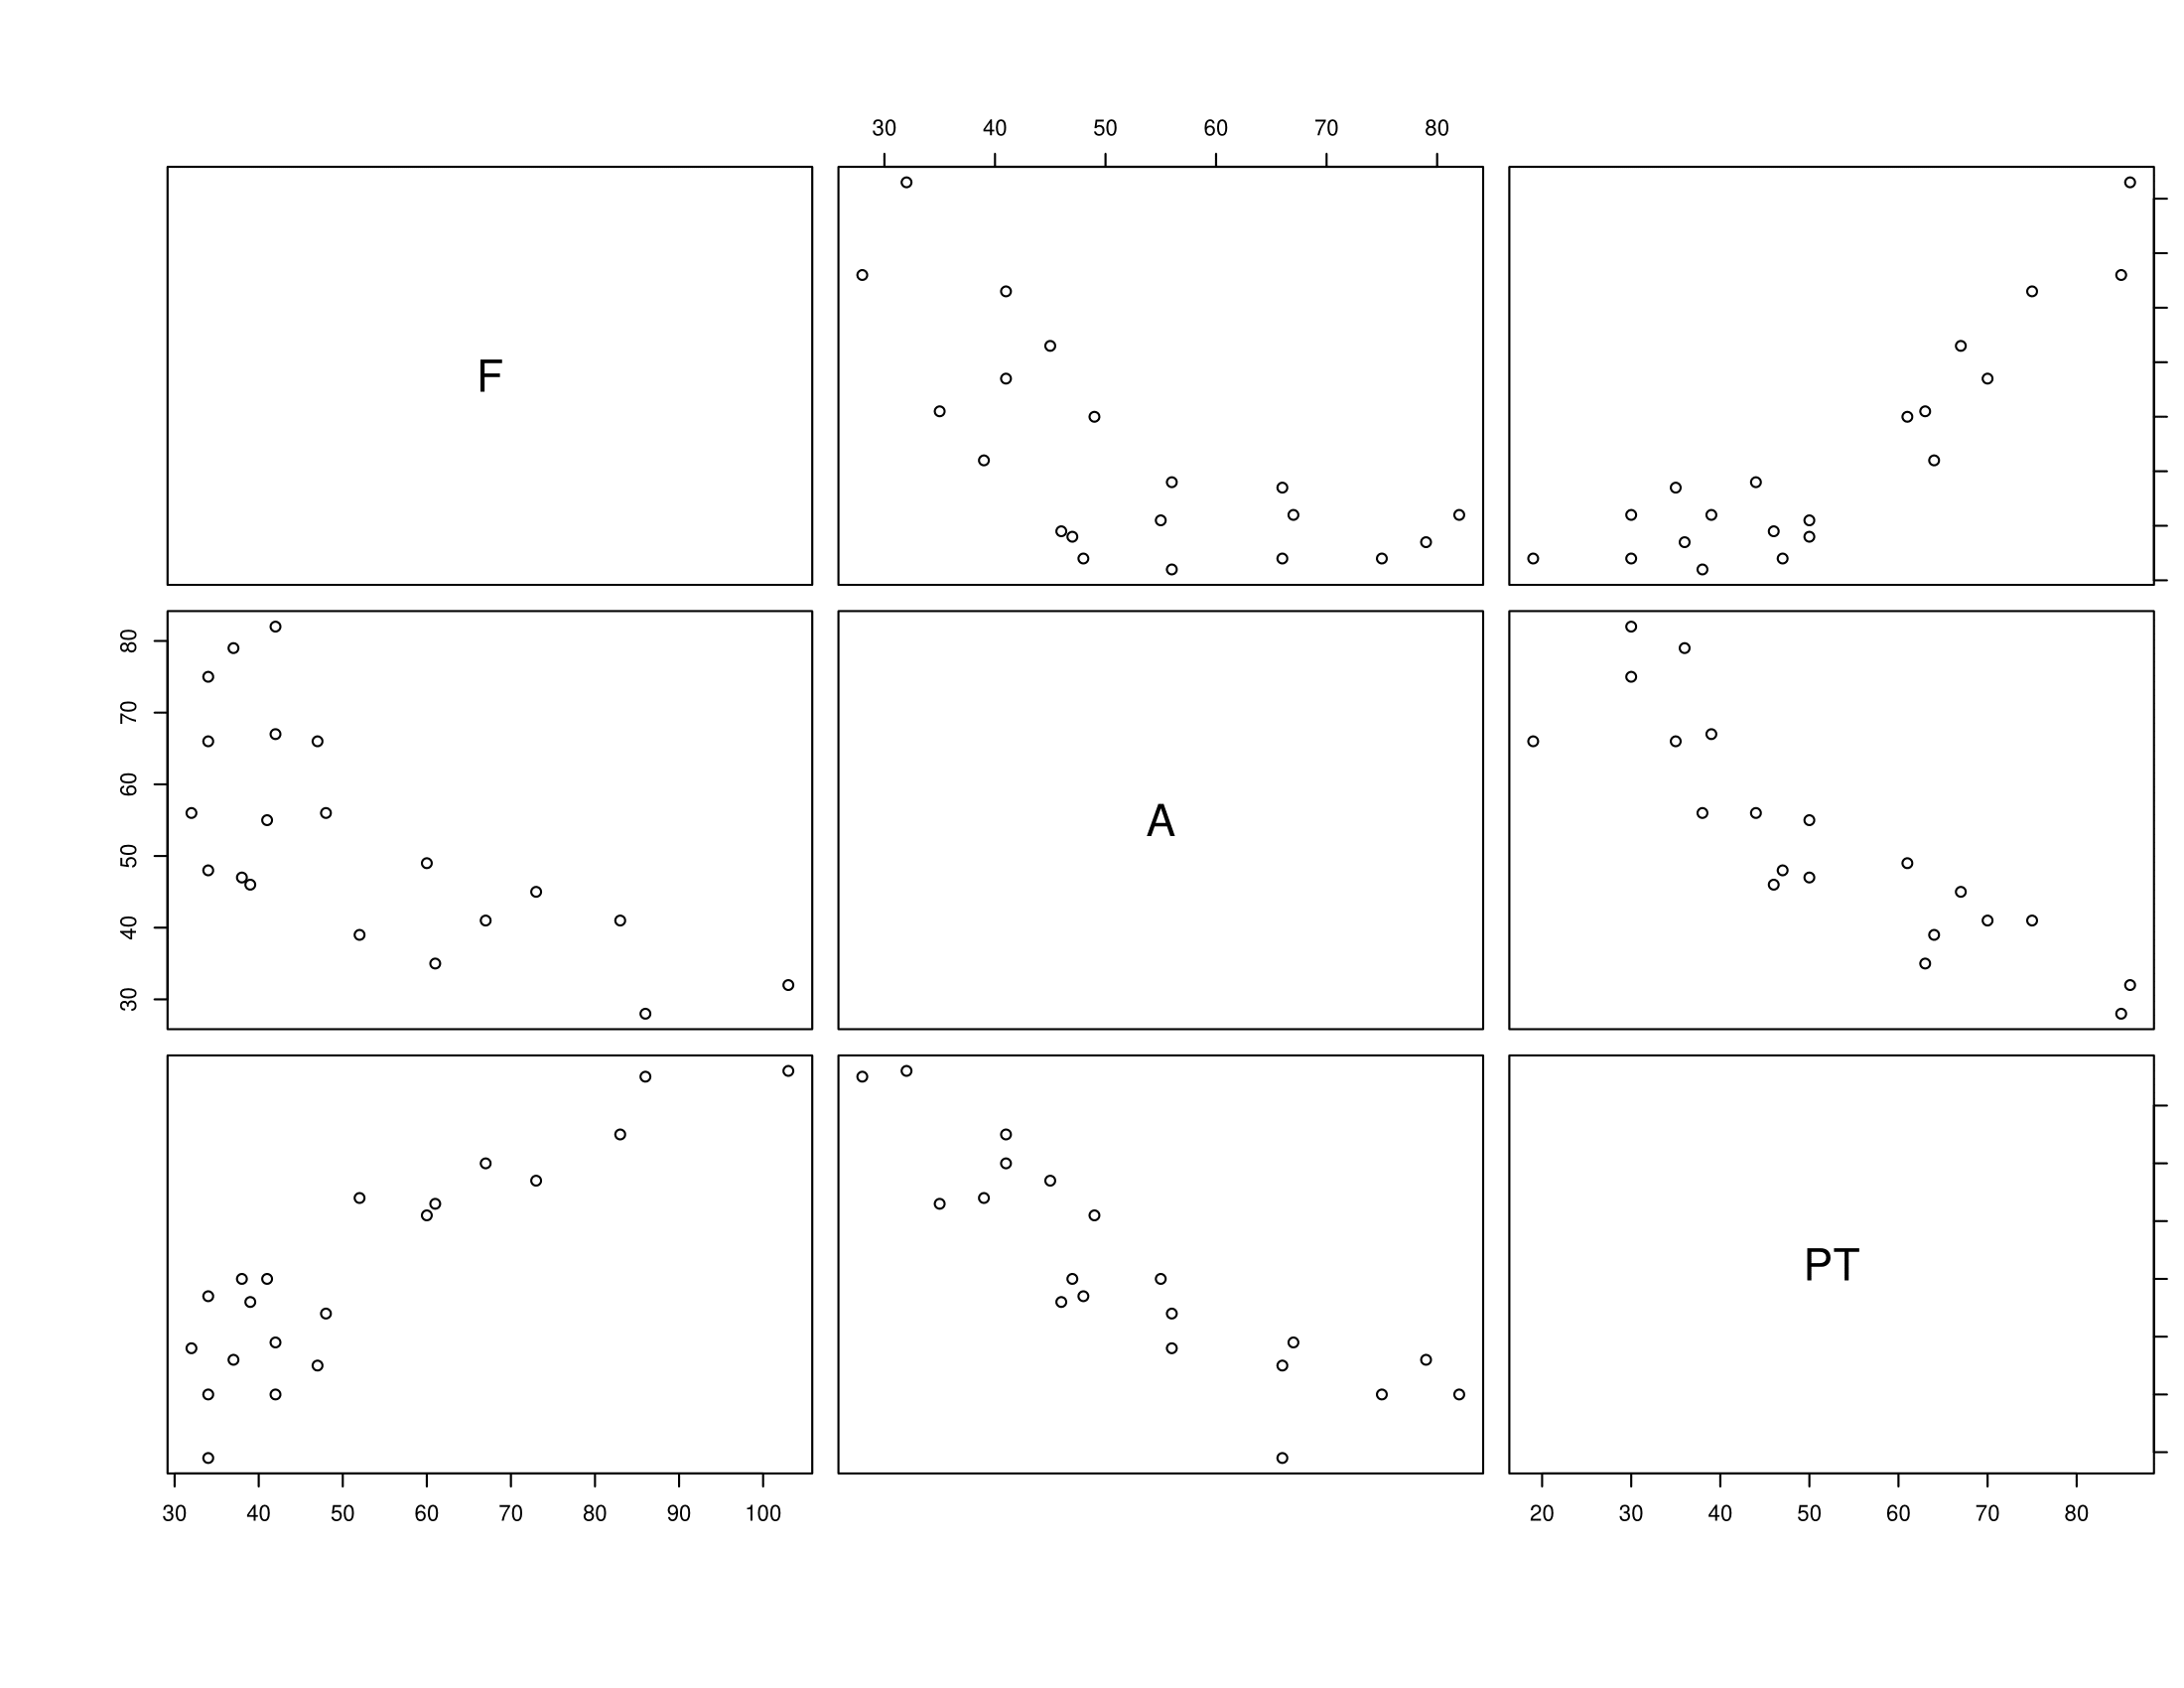
\includegraphics{figs/pairs.png}

You can also use the \texttt{plot3d} command in the \texttt{rgl} library to create an interactive 3D plot of the data. The difficulty of displaying multivariate data is further motivation for developing a method for reducing the number of dimensions in the data.

\hypertarget{random-vectors-and-matrices}{%
\section{Random Vectors and Matrices}\label{random-vectors-and-matrices}}

\begin{definition}
\protect\hypertarget{def:popmean}{}{\label{def:popmean} }The \textbf{population mean vector} of the random vector \(\boldsymbol x\) is
\[\boldsymbol \mu= {\mathbb{E}}(\boldsymbol x).\]

The \textbf{population covariance matrix} of \(\boldsymbol x\) is
\[ \boldsymbol \Sigma= {\mathbb{V}\operatorname{ar}}(\boldsymbol x) = {\mathbb{E}}\left((\boldsymbol x-{\mathbb{E}}(\boldsymbol x))(\boldsymbol x-{\mathbb{E}}(\boldsymbol x))^\top \right).\]

The \textbf{covariance} between \(\boldsymbol x\) (\(p \times 1\)) and \(\boldsymbol y\) (\(q \times 1\)) is
\[ {\mathbb{C}\operatorname{ov}}(\boldsymbol x,\boldsymbol y) = {\mathbb{E}}\left((\boldsymbol x- {\mathbb{E}}(\boldsymbol x))(\boldsymbol y- {\mathbb{E}}(\boldsymbol y))^\top \right). \]
\end{definition}

Let \(\boldsymbol A\) denote a \(q \times p\) constant matrix, and let \(\boldsymbol b\) a constant vector of size \(q \times 1\).
Expectation is a linear operator in the sense that

\[{\mathbb{E}}(\boldsymbol A\boldsymbol x+ \boldsymbol b) = \boldsymbol A{\mathbb{E}}(\boldsymbol x) + \boldsymbol b=\boldsymbol A\boldsymbol \mu+\boldsymbol b.\]

The following properties follow:

\begin{itemize}
\tightlist
\item
  \({\mathbb{V}\operatorname{ar}}(\boldsymbol x) = {\mathbb{E}}(\boldsymbol x\boldsymbol x^\top) - \boldsymbol \mu\boldsymbol \mu^\top\).
\item
  \({\mathbb{V}\operatorname{ar}}(\boldsymbol A\boldsymbol x+ \boldsymbol b) = \boldsymbol A\boldsymbol \Sigma\boldsymbol A^\top\)
\item
  \({\mathbb{C}\operatorname{ov}}(\boldsymbol x,\boldsymbol y) = {\mathbb{E}}(\boldsymbol x\boldsymbol y^\top) - {\mathbb{E}}(\boldsymbol x) {\mathbb{E}}(\boldsymbol y)^\top\).
\item
  \({\mathbb{C}\operatorname{ov}}(\boldsymbol x,\boldsymbol x) = \boldsymbol \Sigma\).
\item
  \({\mathbb{C}\operatorname{ov}}(\boldsymbol x,\boldsymbol y) = {\mathbb{C}\operatorname{ov}}(\boldsymbol y,\boldsymbol x)^\top\).
\item
  \({\mathbb{C}\operatorname{ov}}(\boldsymbol A\boldsymbol x,\boldsymbol B\boldsymbol y) = \boldsymbol A{\mathbb{C}\operatorname{ov}}(\boldsymbol x,\boldsymbol y)\boldsymbol B^\top\)
\item
  If \(p=q\) then
  \[
  {\mathbb{V}\operatorname{ar}}(\boldsymbol x+ \boldsymbol y) = {\mathbb{V}\operatorname{ar}}(\boldsymbol x) + {\mathbb{V}\operatorname{ar}}(\boldsymbol y) + {\mathbb{C}\operatorname{ov}}(\boldsymbol x,\boldsymbol y) + {\mathbb{C}\operatorname{ov}}(\boldsymbol y,\boldsymbol x).
  \]
\end{itemize}

Finally, note that if \(\boldsymbol x\) and \(\boldsymbol y\) are independent (in which case I will write \(\boldsymbol x\perp \!\!\! \perp\boldsymbol y\)) then \({\mathbb{C}\operatorname{ov}}(\boldsymbol x,\boldsymbol y) = {\mathbf 0}_{p,q}\), i.e., a \(p\times q\) matrix of zeros.

\hypertarget{unbiased-estimators}{%
\section{Unbiased Estimators}\label{unbiased-estimators}}

\begin{definition}
\protect\hypertarget{def:unnamed-chunk-11}{}{\label{def:unnamed-chunk-11} }For a staistical model \(p(x\mid \theta)\), a statistic \(\hat{\theta}\equiv\hat{\theta}(X)\) is said to be an \textbf{unbiased estimator} of \(\theta\) if \({\mathbb{E}}_{x\mid \theta}(\hat{\theta}(X)) = \theta\) for all \(\theta\).
\end{definition}

I.e., if data are generated with parameter value \(\theta\), then an estimator \(\hat{\theta}\) is an unbiased estimator of \(\theta\) if its expected value matches the true value (the value used to generate the data).
This concept readily transfers to the multivariate context.

\begin{proposition}
\protect\hypertarget{prp:unnamed-chunk-12}{}{\label{prp:unnamed-chunk-12} }Let \(\boldsymbol x_1, \ldots \boldsymbol x_n\) be independent and identically distributed (i.i.d.), sampled from a population with mean \(\boldsymbol \mu\) and covariance matrix \(\boldsymbol \Sigma\). If \(\bar{\boldsymbol x}\) and \(\boldsymbol S\) are the sample mean and covariance matrix respectively, then

\begin{enumerate}
\def\labelenumi{\arabic{enumi}.}
\item
  \({\mathbb{E}}(\bar{\boldsymbol x}) = \boldsymbol \mu\).
\item
  \({\mathbb{V}\operatorname{ar}}(\bar{\boldsymbol x}) = {\displaystyle\frac{1}{n}} \boldsymbol \Sigma\).
\item
  \({\mathbb{E}}(\boldsymbol S) = {\displaystyle\frac{n-1}{n}} \boldsymbol \Sigma\).
\end{enumerate}
\end{proposition}

\begin{proof}
\iffalse{} {Proof. } \fi{}\textbf{Part 1} By the linearity of expectation,
\[{\mathbb{E}}(\bar{\boldsymbol x}) = {\mathbb{E}}\left(\frac{1}{n} \sum_{i=1}^n \boldsymbol x_i \right)= \frac{1}{n} \sum_{i=1}^n {\mathbb{E}}(\boldsymbol x_i) = \frac{1}{n} n \boldsymbol \mu= \boldsymbol \mu.\]
\textbf{Part 2}
We have
\begin{eqnarray*}
{\mathbb{V}\operatorname{ar}}(\bar{\boldsymbol x}) &=& {\mathbb{V}\operatorname{ar}}\left(\frac{1}{n} \sum_{i=1}^n \boldsymbol x_i \right)\\
&=& \sum_{i,j=1}^n {\mathbb{C}\operatorname{ov}}\left (\frac{1}{n}\boldsymbol x_i, \frac{1}{n}\boldsymbol x_j \right)\\
&=& \sum_{i=1}^n {\mathbb{V}\operatorname{ar}}\left(\frac{1}{n} \boldsymbol x_i \right)+ \sum_{i \neq j} {\mathbb{C}\operatorname{ov}}\left(\frac{1}{n} \boldsymbol x_i, \frac{1}{n} \boldsymbol x_j \right)\\
&=& \frac{1}{n^2} \left(\sum_{i=1}^n {\mathbb{V}\operatorname{ar}}(\boldsymbol x_i) + \sum_{i \neq j} {\mathbb{C}\operatorname{ov}}(\boldsymbol x_i,\boldsymbol x_j) \right)\\
&=& \frac{1}{n^2} \left(\sum_{i=1}^n {\mathbb{V}\operatorname{ar}}(\boldsymbol x_i) \right)\mbox{ as } \boldsymbol x_i \perp \!\!\! \perp\boldsymbol x_j \mbox{ for } i\not = j\\
&=& \frac{1}{n^2} n \boldsymbol \Sigma\\
&=& \frac{1}{n} \boldsymbol \Sigma.
\end{eqnarray*}

\textbf{Part 3} From the definition of the sample covariance,
\begin{eqnarray*}
\boldsymbol S&=& \frac{1}{n} \sum_{i=1}^n  (\boldsymbol x_i -\bar{\boldsymbol x})( \boldsymbol x_i - \bar{\boldsymbol x})^\top \\
&=& \frac{1}{n} \sum_{i=1}^n (\boldsymbol x_i - \boldsymbol \mu+ \boldsymbol \mu-\bar{\boldsymbol x})(\boldsymbol x_i - \boldsymbol \mu+\boldsymbol \mu-\bar{\boldsymbol x})^\top  \\
&=& \frac{1}{n} \sum_{i=1}^n \bigg \{(\boldsymbol x_i - \boldsymbol \mu)(\boldsymbol x_i - \boldsymbol \mu)^\top +(\bar{\boldsymbol x}-\boldsymbol \mu)(\bar{\boldsymbol x}-\boldsymbol \mu)^\top \\
&&  \qquad -(\boldsymbol x_i-\boldsymbol \mu)(\bar{\boldsymbol x}-\boldsymbol \mu)^\top -(\bar{\boldsymbol x}-\boldsymbol \mu)(\boldsymbol x_i-\boldsymbol \mu)^\top \bigg \}\\
&=& \frac{1}{n} \left \{\sum_{i=1}^n (\boldsymbol x_i - \boldsymbol \mu)(\boldsymbol x_i - \boldsymbol \mu)^\top \right \}- (\bar{\boldsymbol x}-\boldsymbol \mu)(\bar{\boldsymbol x}-\boldsymbol \mu)^\top
\end{eqnarray*}
as \(\frac{1}{n}\sum (\bar{\boldsymbol x}-\boldsymbol \mu)(\boldsymbol x_i-\boldsymbol \mu)^\top = \sum (\bar{\boldsymbol x}-\boldsymbol \mu)(\bar{\boldsymbol x} -\boldsymbol \mu)^\top\).
Since \({\mathbb{E}}(\bar{\boldsymbol x})=\boldsymbol \mu\) and \({\mathbb{V}\operatorname{ar}}(\bar{\boldsymbol x})=n^{-1}\boldsymbol \Sigma\), it follows that

\begin{eqnarray*}
{\mathbb{E}}(\boldsymbol S)&=&\left \{\frac{1}{n}\sum_{i=1}^n {\mathbb{E}}\left [(\boldsymbol x_i - \boldsymbol \mu)(\boldsymbol x_i - \boldsymbol \mu)^\top \right ]\right \} -{\mathbb{V}\operatorname{ar}}(\bar{\boldsymbol x})\\
&=&{\mathbb{E}}\left \{(\boldsymbol x_1 - \boldsymbol \mu)(\boldsymbol x_1  - \boldsymbol \mu)^\top \right \} -{\mathbb{V}\operatorname{ar}}(\bar{\boldsymbol x})\\
&=& {\mathbb{V}\operatorname{ar}}(\boldsymbol x_1)-{\mathbb{V}\operatorname{ar}}(\bar{\boldsymbol x}) \\
&=& \boldsymbol \Sigma- \frac{1}{n}\boldsymbol \Sigma\\
&=& \frac{n-1}{n}  \boldsymbol \Sigma,
\end{eqnarray*}

which completes the proof.\\
\end{proof}

An implication of this theorem is that \(\bar{\boldsymbol x}\) is an unbiased estimator for \(\boldsymbol \mu\) but that \(\boldsymbol S\) is a biased estimator of \(\boldsymbol \Sigma\). Note, however, that \({\displaystyle\frac{n}{n-1}} \boldsymbol S\) is an unbiased estimator of \(\boldsymbol \Sigma\), i.e.
\[
 \frac{n}{n-1}{\mathbb{E}}[\boldsymbol S]=\boldsymbol \Sigma.
 \]

\hypertarget{linalg-prelim}{%
\chapter{Review of linear algebra}\label{linalg-prelim}}

Modern statistics and machine learning rely heavily upon linear algebra, nowhere more so than in multivariate statistics. In the first part of this chapter (sections \ref{linalg-basics} and \ref{linalg-vecspaces}) we review some concepts from linear algebra that will be needed throughout the module, including vector spaces, row and column spaces, the rank of a matrix, etc. Hopefully most of this will be familiar to you.

We then cover some basic details on inner-product or normed spaces in \ref{linalg-innerprod}, which are vector spaces equipped with a concept of distance and angle.

Section \ref{linalg-decomp} is perhaps the most important section. Here we provide a reminder about eigenvalues and the spectral decomposition of square symmetric matrices, before introducing the singular value decomposition (SVD) in Section \ref{linalg-SVD}. The SVD is one of the most important concepts in this module, and is the key linear algebra technique behind many of the methods we will study. Finally, in Section \ref{linalg-misc} we will cover some miscellaneous topics that will be needed in later chapters.

I do not provide proofs of all the results stated in this chapter, but instead prove a small selection which I think it is useful to see. For a complete treatment of the linear algebra needed for this module, see the excellent book ``Linear algebra and learning from data'' by Gilbert Strang.

I have recorded videos on some (but not all) of the topics in these notes:

\begin{itemize}
\tightlist
\item
  \href{https://mediaspace.nottingham.ac.uk/media/Vector+Spaces/1_48xqrp04}{Vector spaces}
\item
  \href{https://mediaspace.nottingham.ac.uk/media/Matrices/1_nqo2u7zs}{Matrices}
\item
  \href{https://mediaspace.nottingham.ac.uk/media/Inner+Product+Spaces/1_nhcbybg3}{Inner product spaces}
\item
  \href{https://mediaspace.nottingham.ac.uk/media/Orthogonal+Matrices/1_rr2ervcs}{Orthogonal matrices}
\item
  \href{https://mediaspace.nottingham.ac.uk/media/Projection/1_soh726fg}{Projection matrices}
\end{itemize}

NOT DONE A VIDEO ON CENTERING MATRIX, OR ELLIPSES, or VECTOR DIFFERENTIATION.

\renewcommand{\bY}{\boldsymbol Y}
\renewcommand{\bx}{\boldsymbol x}
\renewcommand{\bX}{\boldsymbol X}
\renewcommand{\bH}{\boldsymbol H}
\renewcommand{\by}{\boldsymbol y}
\renewcommand{\bz}{\boldsymbol z}
\renewcommand{\bS}{\boldsymbol S}
\renewcommand{\bR}{\boldsymbol R}
\renewcommand{\bmu}{\boldsymbol \mu}
\renewcommand{\bSigma}{\boldsymbol \Sigma}
\renewcommand{\bLambda}{\boldsymbol \Lambda}
\renewcommand{\bgamma}{\boldsymbol \gamma}
\renewcommand{\blambda}{\boldsymbol \lambda}
\renewcommand{\bA}{\boldsymbol A}
\renewcommand{\bB}{\boldsymbol B}
\renewcommand{\bD}{\boldsymbol D}
\renewcommand{\bC}{\boldsymbol C}
\renewcommand{\bR}{\boldsymbol R}
\renewcommand{\bM}{\boldsymbol M}
\renewcommand{\bP}{\boldsymbol P}
\renewcommand{\bQ}{\boldsymbol Q}
\renewcommand{\bT}{\boldsymbol T}
\renewcommand{\bW}{\boldsymbol W}
\renewcommand{\ba}{\boldsymbol a}
\renewcommand{\bb}{\boldsymbol b}
\renewcommand{\bc}{\boldsymbol c}
\renewcommand{\bd}{\boldsymbol d}
\renewcommand{\bh}{\boldsymbol h}
\renewcommand{\bp}{\boldsymbol p}
\renewcommand{\bq}{\boldsymbol q}
\renewcommand{\bu}{\boldsymbol u}
\renewcommand{\bzero}{\boldsymbol 0}
\renewcommand{\mR}{\mathbb R}
\renewcommand{\cR}{\mathcal R}

\renewcommand{\bs}{\boldsymbol}
\renewcommand{\ds}{\displaystyle}
\renewcommand{\tdiag}{\text{diag}}
\renewcommand{\ttr}{\text{tr}}
\renewcommand{\tdet}{\text{det}}

\renewcommand{\tcov}{\text{cov}}
\renewcommand{\texp}{\text{exp}}
\renewcommand{\lb}{\left(}
\renewcommand{\rb}{\right)}
\renewcommand{\lsb}{\left[}
\renewcommand{\rsb}{\right]}

\hypertarget{linalg-basics}{%
\section{Basics}\label{linalg-basics}}

In this section, we recap some basic definitions and notation. Hopefully this material will largely be familiar to you.

\hypertarget{notation}{%
\subsection{Notation}\label{notation}}

The matrix \({\mathbf A}\) will be referred to in the following equivalent ways:
\begin{eqnarray*}
{\mathbf A}=\stackrel{n\times p}{\mathbf A} &=& \left[\begin{array}{cccc}
a_{11}&a_{12}&\dots&a_{1p}\\
a_{21}&a_{22}&\dots&a_{2p}\\
\vdots&\vdots&&\vdots\\
a_{n1}&a_{n2}&\dots&a_{np}
\end{array} \right] \\
&=&[a_{ij}: i=1, \ldots , m; j=1, \ldots , n]\\
&=&(a_{ij})\\
&=& \left[ \begin{array}{c}\boldsymbol a_1^\top\\
\vdots\\
\boldsymbol a_n^\top\end{array}\right]
\end{eqnarray*}
where the \(a_{ij}\) are the individual entries, and \(\boldsymbol a_i^\top=(a_{i1}, a_{i2}, \ldots, a_{ip})\) is the \(i^{th}\) row.

A matrix of order \(1\times 1\) is called a \emph{scalar}.

A matrix of order \(n\times 1\) is called a \emph{(column) vector}.

A matrix of order \(1\times p\) is called a \emph{(row) vector}.

e.g. \(\stackrel{n\times 1}{\mathbf a}=\left( \begin{array}{c} a_1\\\vdots\\a_n \end{array} \right)\)\quad is a column vector.

The \(n\times n\) \emph{identity matrix} \({\mathbf I}_n\) has diagonal elements equal to 1
and off-diagonal elements equal to zero.

A \emph{diagonal} matrix is an \(n \times n\) matrix whose
off-diagonal elements are zero. Sometimes we denote a diagonal
matrix by \(\text{diag}\{a_1,\ldots, a_n\}\).

\[\mathbf I_3 = \left(\begin{array}{ccc} 1&0&0\\ 0&1&0\\ 0&0&1\end{array}\right),\quad \text{diag}\{1,2,3\}=\left(\begin{array}{ccc} 1&0&0\\ 0&2&0\\ 0&0&3\end{array}\right)\quad\]

\hypertarget{elementary-matrix-operations}{%
\subsection{Elementary matrix operations}\label{elementary-matrix-operations}}

\begin{enumerate}
\def\labelenumi{\arabic{enumi}.}
\item
  \emph{Addition/Subtraction}. If \(\stackrel{n\times p}{\mathbf A}=[a_{ij}]\) and \(\stackrel{n\times p}{\mathbf B}=[b_{ij}]\) are
  given matrices then
  \[ {\mathbf A}+{\mathbf B}=[a_{ij}+b_{ij}] \qquad \text{and} \qquad {\mathbf A}-{\mathbf B}=[a_{ij}-b_{ij}].\]
\item
  \emph{Scalar Multiplication}. If \(\lambda\) is a scalar and \({\mathbf A}=[a_{ij}]\) then
  \[\lambda {\mathbf A}=[\lambda a_{ij}].\]
\item
  \emph{Matrix Multiplication}. If \(\stackrel{n\times p}{\mathbf A}\) and \(\stackrel{p\times q}{\mathbf B}\) are
  matrices then \(\boldsymbol A\boldsymbol B=\stackrel{n\times q}{\mathbf C}=[c_{ij}]\) where
  \[c_{ij}=\sum _{k=1}^p a_{ik}b_{kj}, \qquad i=1,\dots,n, \qquad j=1,\dots ,q.\]
\item
  \emph{Matrix Transpose}. If \(\stackrel{m \times n}{\boldsymbol A}=[a_{ij}: i=1, \ldots , m; j=1, \ldots , n]\), then the transpose of \(\boldsymbol A\), written
  \(\boldsymbol A^\top\), is given by the \(n \times m\) matrix
  \[
  \boldsymbol A^\top =[a_{ji}: j=1, \ldots , n; i=1, \ldots, m].
  \]
  Note from the definitions that \((\boldsymbol A\boldsymbol B)^\top={\mathbf B}^\top {\mathbf A}^\top\).
\item
  \emph{Matrix Inverse}. The inverse of a matrix \(\stackrel{n\times n}{\mathbf A}\) (if it exists) is a
  matrix \(\stackrel{n\times n}{\mathbf B}\) such that \({\mathbf A}\boldsymbol B=\boldsymbol B\boldsymbol A={\mathbf I}_n.\) We denote
  the inverse by \({\mathbf A}^{-1}\). Note that if \({\mathbf A}_1\) and \({\mathbf A}_2\) are both invertible,
  then \(({\mathbf A}_1 {\mathbf A}_2)^{-1}={\mathbf A}_2^{-1}{\mathbf A}_1^{-1}\).
\item
  \emph{Trace}. The trace of a matrix \(\stackrel{n\times n}{\mathbf A}\) is given by
  \[ \text{tr}({\mathbf A})=\sum _{i=1}^n a_{ii}.\]
\end{enumerate}

\begin{lemma}
\protect\hypertarget{lem:unnamed-chunk-1}{}{\label{lem:unnamed-chunk-1} }For any matrices \(\boldsymbol A\) (\(n \times m\)) and \(\boldsymbol B\) (\(m \times n\)),
\[
\text{tr}(\boldsymbol A\boldsymbol B) = \text{tr}(\boldsymbol B\boldsymbol A).
\]
\end{lemma}

\begin{enumerate}
\def\labelenumi{\arabic{enumi}.}
\setcounter{enumi}{6}
\tightlist
\item
  The \emph{determinant} of a square matrix \(\stackrel{n\times n}{\mathbf A}\) is
  defined as
  \[ \text{det}({\mathbf A})=\sum (-1)^{|\tau |} a_{1\tau(1)}\dots a_{n\tau (n)} \]
  where the summation is taken over all permutations \(\tau\) of \(\{1,2,\dots ,n\}\),
  and we define \(|\tau |=0\) or \(1\) depending on whether \(\tau\) can be written as an even or
  odd number of transpositions.
\end{enumerate}

E.g. If \({\mathbf A}=\left[ \begin{array}{cc} a_{11}&a_{12}\\ a_{21}&a_{22} \end{array} \right]\),
then \(\text{det}({\mathbf A})=a_{11}a_{22}-a_{12}a_{21}\).

\begin{proposition}
\protect\hypertarget{prp:det1}{}{\label{prp:det1} }Matrix \(\stackrel{n\times n}{\mathbf A}\) is invertible if and only if \(\det(\boldsymbol A)\not = 0\). If \(\boldsymbol A^{-1}\) exists then
\[\det(\boldsymbol A)=\frac{1}{\det(\boldsymbol A^{-1})}\]
\end{proposition}

\begin{proposition}
\protect\hypertarget{prp:det3}{}{\label{prp:det3} }For any matrices \(\stackrel{n\times n}{\mathbf A}\),
\(\stackrel{n\times n}{\mathbf B}\), \(\stackrel{n\times n}{\mathbf C}\) such that \({\mathbf C}={\mathbf{AB}}\),
\[ \text{det}({\mathbf C})=\text{det}({\mathbf A}) \cdot \text{det}({\mathbf B}).\]
\end{proposition}

\hypertarget{special-matrices}{%
\subsection{Special matrices}\label{special-matrices}}

\begin{definition}
\protect\hypertarget{def:posdef}{}{\label{def:posdef} }An \(n\times n\) matrix \(\boldsymbol A\) is symmetric if
\[\boldsymbol A= \boldsymbol A^\top.\]
An \(n\times n\) symmetric matrix \(\boldsymbol A\) is \textbf{positive-definite} if
\[\boldsymbol x^\top \boldsymbol A\boldsymbol x>0 \mbox{ for all } \boldsymbol x\in \mathbb{R}^n, \boldsymbol x\not = \boldsymbol 0\]
and is \textbf{positive semi-definite} if
\[\boldsymbol x^\top \boldsymbol A\boldsymbol x\geq 0 \mbox{ for all } \boldsymbol x\in \mathbb{R}^n.\]

\(\boldsymbol A\) is \textbf{idempotent} if \(\boldsymbol A^2=\boldsymbol A\).
\end{definition}

\hypertarget{vector-differentiation}{%
\subsection{Vector Differentiation}\label{vector-differentiation}}

Consider a real-valued function \(f: \mathbb{R}^p \rightarrow \mathbb{R}\) of a vector variable \(\boldsymbol x=(x_1, \ldots , x_p)^\top\). Sometimes we will want to differentiate \(f\). We define the partial derivative of \(f(\boldsymbol x)\) with respect to \(\boldsymbol x\) to be
the vector of partial derivatives, i.e.
\begin{equation}
\frac{\partial f}{\partial \boldsymbol x}(\boldsymbol x)=\left [ \begin{array}{c} \frac{\partial f}{\partial x_1}(\boldsymbol x)\\
 ..\\
 ..\\
 ..\\
 \frac{\partial f}{\partial x_p}(\boldsymbol x)
\end{array} \right ]
\label{eq:derivx}
\end{equation}
The following examples can be worked out directly from the definition \eqref{eq:derivx}, using the chain rule in some cases.

\begin{example}
\protect\hypertarget{exm:calc1}{}{\label{exm:calc1} }If \(f(\boldsymbol x)=\boldsymbol a^\top \boldsymbol x\) where \(\boldsymbol a\in \mathbb{R}^p\) is a constant vector, then
\[
\frac{\partial f}{\partial \boldsymbol x}(\boldsymbol x)=\boldsymbol a.
\]
\end{example}

\begin{example}
\protect\hypertarget{exm:calc2}{}{\label{exm:calc2} }If \(f(\boldsymbol x)=(\boldsymbol x-\boldsymbol a)^\top \boldsymbol A(\boldsymbol x-\boldsymbol a)\) for a fixed vector \(\boldsymbol a\in \mathbb{R}^p\)
and \(\boldsymbol A\) is a symmetric constant \(p \times p\) matrix, then
\[
\frac{\partial f}{\partial \boldsymbol x}(\boldsymbol x)=2\boldsymbol A(\boldsymbol x-\boldsymbol a).
\]
\end{example}

\begin{example}
\protect\hypertarget{exm:calc3}{}{\label{exm:calc3} }Suppose that \(g: \, \mathbb{R} \rightarrow \mathbb{R}\) is a differentiable function with derivative \(g^\prime\). Then, using the chain rule for partial derivatives,
\[
\frac{\partial g(\boldsymbol a^\top \boldsymbol x)}{\partial \boldsymbol x}=g^{\prime}(\boldsymbol a^\top\boldsymbol x)\frac{\partial}{\partial \boldsymbol x}\left \{\boldsymbol a^\top \boldsymbol x\right \}=g^{\prime}(\boldsymbol a^\top\boldsymbol x) \boldsymbol a.
\]
\end{example}

\begin{example}
\protect\hypertarget{exm:calc4}{}{\label{exm:calc4} }If \(f\) is defined as in Example \ref{exm:calc2} and \(g\) is as in Example \ref{exm:calc3} then, using the chain rule again,
\[
\frac{\partial }{\partial \boldsymbol x} g\{f(\boldsymbol x)\}=g^{\prime} \{f(\boldsymbol x)\}\frac{\partial f}{\partial \boldsymbol x}(\boldsymbol x)
=2 g^{\prime}\{(\boldsymbol x- \boldsymbol a)^\top \boldsymbol A(\boldsymbol x- \boldsymbol a)\}\boldsymbol A(\boldsymbol x-\boldsymbol a).
\]
\end{example}

If we wish to find a maximum or minimum of \(f(\boldsymbol x)\) we should search for stationary points of \(f\),
i.e.~solutions to the system of equations
\[
\frac{\partial f}{\partial \boldsymbol x}(\boldsymbol x)\equiv \left [ \begin{array}{c} \frac{\partial f}{\partial x_1}(\boldsymbol x)\\
 ..\\
 ..\\
 ..\\
 \frac{\partial f}{\partial x_p}(\boldsymbol x)
\end{array} \right ]={\mathbf 0}_p.
\]
\begin{definition}
\protect\hypertarget{def:hessian}{}{\label{def:hessian} }The \textbf{Hessian} matrix of \(f\) is the \(p \times p\) matrix of second derivatives.
\[
\frac{\partial^2f}{\partial \boldsymbol x\partial \boldsymbol x^\top}(\boldsymbol x) =\left \{ \frac{\partial^2 f(\boldsymbol x)}{\partial x_j \partial x_k}\right \}_{j,k=1}^p.
\]
\end{definition}

The nature of a stationary point is determined by the Hessian

If the Hessian is positive (negative) definite at a stationary point \(\boldsymbol x\), then the stationary point is a minimum (maximum).

If the Hessian has both positive and negative eigenvalues at \(\boldsymbol x\) then the stationary point will be a \emph{saddle point}.

\hypertarget{linalg-vecspaces}{%
\section{Vector spaces}\label{linalg-vecspaces}}

It will be useful to talk about \textbf{vector spaces}. These are sets of vectors that can be added together, or multiplied by a scalar. You should be familiar with these from your undergraduate degree. We don't provide a formal definition here, but you can think of a real vector space \(V\) as a set of vectors such that for any \(\boldsymbol v_1, \boldsymbol v_2 \in V\) and \(\alpha_1, \alpha_2 \in \mathbb{R}\), we have
\[\alpha_1 \boldsymbol v_1 + \alpha_2 \boldsymbol v_2 \in V\]
i.e., vector spaces are closed under addition and scalar multiplication.

\begin{example}
\protect\hypertarget{exm:Rp}{}{\label{exm:Rp} }Euclidean space in \(p\) dimensions, \(\mathbb{R}^p\), is a vector space. If we add any two vectors in \(\mathbb{R}^p,\) or multiply a vector by a real scalar, then the resulting vector also lies in \(\mathbb{R}^p\).
\end{example}

A subset \(U \subset V\) of a vector space \(V\) is called a vector \textbf{subspace} if \(U\) is also a vector space.

\begin{example}
\protect\hypertarget{exm:Rp2}{}{\label{exm:Rp2} }Let \(V=\mathbb{R}^2\). Then the sets \[U_1 = \left\{\left(
        \begin{array}{c}
        a\\
      0  \end{array}
        \right): a\in \mathbb{R}\right\}, \mbox{ and}\quad U_2 = \left\{a\left(
        \begin{array}{c}
       1 \\
      1  \end{array}
        \right): a\in \mathbb{R}\right\}\]
are both subspaces of \(V\).
\end{example}

\hypertarget{linear-independence}{%
\subsection{Linear independence}\label{linear-independence}}

\begin{definition}
\protect\hypertarget{def:linindep}{}{\label{def:linindep} }Vectors \(\stackrel{n\times 1}{\mathbf x}_1 ,\dots , \stackrel{n\times 1}{\mathbf x}_p\)
are said to be \textbf{linearly dependent} if there exist scalars
\(\lambda _1, \dots ,\lambda _p\) not all zero such that
\[ \lambda _1 {\mathbf x}_1+\lambda _2 {\mathbf x}_2+ \dots + \lambda _p {\mathbf x}_p={\mathbf 0}.\]
Otherwise, these vectors are said to be \textbf{linearly independent}.
\end{definition}

\begin{definition}
\protect\hypertarget{def:span}{}{\label{def:span} }Given a set of vectors \(S=\{s_1, \ldots, s_n\}\), the \textbf{span} of \(S\) is the smallest vector space containing \(S\) or equivalently, is the set of all linear combinations of vectors from \(S\)
\[\operatorname{span}(S) = \left\{ \sum_{i=1}^k \alpha_i s_i \mid k \in \mathbb{N}, \alpha_i \in \mathbb{R}, s_i \in S\right\}\]
\end{definition}

\begin{definition}
\protect\hypertarget{def:basis}{}{\label{def:basis} }A \textbf{basis} of a vector space \(V\) is a set of linearly independent vectors in \(V\) that span \(V\).
\end{definition}

\begin{example}
\protect\hypertarget{exm:basisRp}{}{\label{exm:basisRp} }Consider \(V=\mathbb{R}^2\). Then the following are both bases for \(V\):
\[B_1=\left\{\left(\begin{array}{c}1\\0\end{array}\right), \left(\begin{array}{c}0\\1\end{array}\right)\right\}
\]
\[B_2=\left\{\left(\begin{array}{c}1\\1\end{array}\right), \left(\begin{array}{c}1\\2\end{array}\right)\right\}
\]\\
\end{example}

\begin{definition}
\protect\hypertarget{def:dimension}{}{\label{def:dimension} }The \textbf{dimension} of a vector space is the number of vectors in its basis.
\end{definition}

\hypertarget{colsspace}{%
\subsection{Row and column spaces}\label{colsspace}}

We can think about the matrix-vector multiplication \(\boldsymbol A\boldsymbol x\) in two ways. The usual way is as the inner product between the rows of \(A\) and \(x\).

\[ \left( \begin{array}{cc} 1 & 2\\ 3&4\\5&6\end{array}\right) \left(\begin{array}{c}x_1\\ x_2\end{array}\right) = \left(\begin{array}{c} x_1+2x_2\\3x_1+4x_2\\5x_1+6x_2\end{array}\right)\]

But a better way to think of \(\boldsymbol A\boldsymbol x\) is as a linear combination of the columns of \(A\).

\[ \left( \begin{array}{cc} 1 & 2\\ 3&4\\5&6\end{array}\right) \left(\begin{array}{c}x_1\\ x_2\end{array}\right) = x_1\left(\begin{array}{c}1\\3\\5 \end{array}\right)+x_2\left(\begin{array}{c}2\\4\\6 \end{array}\right)\]

\begin{definition}
\protect\hypertarget{def:rank}{}{\label{def:rank} }The \textbf{column space} of a \(n\times p\) matrix \(\boldsymbol A\) is the set of all linear combinations of the columns of \(\boldsymbol A\):
\[\mathcal{C}(\boldsymbol A) = \{\boldsymbol A\boldsymbol x:  \boldsymbol x\in \mathbb{R}^p\}\subset \mathbb{R}^n\]
\end{definition}

For \[A=\left( \begin{array}{cc} 1 & 2\\ 3&4\\5&6\end{array}\right) \] we can see that the column space is a 2-dimensional plane in \(\mathbb{R}^3\). The matrix \(\boldsymbol B\) has the same column space as \(\boldsymbol A\)
\[\boldsymbol B=\left( \begin{array}{cccc} 1 & 2&3 &4\\ 3&4 &7&10\\5&6&11&16\end{array}\right) \]

The number of linearly independent columns of \(\boldsymbol A\) is called the \textbf{column rank} of \(\boldsymbol A\), and is equal to the dimension of the column space of \(\mathcal{C}(\boldsymbol A)\). The \textbf{column rank} of \(\boldsymbol A\) and \(\boldsymbol B\) is 2.

The \textbf{row space} of \(\boldsymbol A\) is defined to be the column space of \(\boldsymbol A^\top\), and the \textbf{row rank} is the number of linearly independent rows of \(\boldsymbol A\).

\begin{theorem}
\protect\hypertarget{thm:rowrank}{}{\label{thm:rowrank} }The \textbf{row rank} of of a matrix equals the \textbf{column rank}.
\end{theorem}

Thus we can simply refer to the \textbf{rank} of the matrix.

\begin{proof}
\iffalse{} {Proof. } \fi{}The proof of this theorem is very simple. Let \(\boldsymbol C\) be an \(n \times r\) matrix (where \(r=\operatorname{rank}(\boldsymbol A)\)) with columns chosen to be a set of \(r\) linearly independent columns from \(A\). Then we know each column of \(\boldsymbol A\) can be written as a linear combination of the columns of \(\boldsymbol C\), i.e.
\[\boldsymbol A= \boldsymbol C\boldsymbol R.\]
The dimension of \(\boldsymbol R\) must be \(r \times p\). But now we can see that the rows of \(\boldsymbol A\) are formed by a linear combination of the rows of \(\boldsymbol R\). Thus the row rank of \(\boldsymbol A\) is at most \(r\) (=the column rank of \(\boldsymbol A\)). This holds for any matrix, so is true for \(\boldsymbol A^\top\): namely \(\operatorname{row-rank}(A^\top)\leq \operatorname{column-rank}(A^\top)\). But the row space of \(\boldsymbol A^\top\) equals \(\mathcal{C}(\boldsymbol A)\), thus proving the theorem!
\end{proof}

\begin{corollary}
\protect\hypertarget{cor:unnamed-chunk-3}{}{\label{cor:unnamed-chunk-3} }The rank of an \(n\times p\) matrix is at most \(\min(n,p)\).
\end{corollary}

\begin{example}
\protect\hypertarget{exm:matrix1}{}{\label{exm:matrix1} }\[B = \left( \begin{array}{cccc} 1 & 2\\ 3&4 \\5&6\end{array}\right)\left(\begin{array}{cccc}1&0&1&2\\0&1&1&1\end{array}\right)
\]
\end{example}

\begin{example}
\protect\hypertarget{exm:matrix2}{}{\label{exm:matrix2} }\[ D=\left( \begin{array}{ccc} 1 & 2&3\\ 2&4&6 \end{array}\right)= \left( \begin{array}{c} 1 \\ 2 \end{array}\right)\left(\begin{array}{ccc}1&2&3\end{array}\right)
\]
So the rank of \(D\) is \(1\).
\end{example}

\hypertarget{linear-transformations}{%
\subsection{Linear transformations}\label{linear-transformations}}

We can view an \(n\times p\) matrix \(\boldsymbol A\) as a linear map between two vector spaces:
\begin{align*}
\boldsymbol A: \;\mathbb{R}^p &\rightarrow   \mathbb{R}^n\\
 \boldsymbol x&\mapsto \boldsymbol A\boldsymbol x
\end{align*}

The \textbf{image} of \(\boldsymbol A\) is precisely the column space of \(\boldsymbol A\):
\[\operatorname{Im}(\boldsymbol A) = \{\boldsymbol A\boldsymbol x: \boldsymbol x\in \mathbb{R}^p\}=\mathcal{C}(\boldsymbol A) \subset \mathbb{R}^n\]

The \textbf{kernel} of \(A\) is the set of vectors mapped to zero:
\[\operatorname{Ker}(\boldsymbol A)=\{\boldsymbol x: \boldsymbol A\boldsymbol x=\boldsymbol 0\}\subset \mathbb{R}^p\]
and is sometimes called the \textbf{null-space} of \(\boldsymbol A\) and denoted \(\mathcal{N}(\boldsymbol A)\).

\begin{theorem}
\protect\hypertarget{thm:ranknullity}{}{\label{thm:ranknullity} }The \textbf{rank-nullity} theorem says if \(V\) and \(W\) are vector spaces, and \(A: V\rightarrow W\) is a linear map, then
\[\dim \operatorname{Im}(A)+\dim \operatorname{Ker}(A) =\dim V\]
\end{theorem}

If we're thinking about matrices, then \(\dim \mathcal{C}(\boldsymbol A)+\dim \mathcal{N}(\boldsymbol A)=p\), or equivalently that\\
\(\operatorname{rank}(\boldsymbol A)+\dim \mathcal{N}(\boldsymbol A)=p\).

We've already said that the row space of \(\boldsymbol A\) is \(\mathcal{C}(\boldsymbol A^\top)\). The left-null space is \(\{\boldsymbol x\in \mathbb{R}^n: \boldsymbol x^\top \boldsymbol A=0\}\) or equivalently \(\{x \in \mathbb{R}^n: \boldsymbol A^\top \boldsymbol x=0\}=\mathcal{N}(\boldsymbol A^\top)\). And so by the rank-nullity theorem we must have
\[n=\dim \mathcal{C}(\boldsymbol A^\top) + \dim \mathcal{N}(\boldsymbol A^\top)=
\operatorname{rank}(\boldsymbol A)+\dim \operatorname{Ker}(\boldsymbol A^\top).\]

\begin{example}
\protect\hypertarget{exm:ranknullityeg}{}{\label{exm:ranknullityeg} }Consider again the matrix \(D: \mathbb{R}^3\rightarrow \mathbb{R}^2\)
\[ D=\left( \begin{array}{ccc} 1 & 2&3\\ 2&4&6 \end{array}\right)= \left( \begin{array}{c} 1 \\ 2 \end{array}\right)\left(\begin{array}{ccc}1&2&3\end{array}\right)
\]
We have already seen that
\[\mathcal{C}(D)=\operatorname{span}\left\{\left(\begin{array}{c}1\\2\end{array}\right)\right\}\]
and so \(\dim \mathcal{C}(D)=\operatorname{rank}(D)=1\).
The kernel, or null-space, of \(\boldsymbol D\) is the set of vectors for which \(\boldsymbol D\boldsymbol x=\boldsymbol 0\), i.e.,
\[x_1+2x_2+3x_3=0\]
This is a single equation with three unknowns, and so there must be a plane of solutions. We need two linearly independent vectors in this plane to describe it. Convince yourself that
\[\mathcal{N}(D) = \operatorname{span}\left\{\left(\begin{array}{c}0\\3\\-2\end{array}\right), \left(\begin{array}{c}2\\-1\\0\end{array}\right)\right\}\]
So we have
\[\dim \mathcal{C}(D)+\dim \mathcal{N}(D)=1+2=3\]
as required by the rank-nullity theorem.

If we consider \(D^\top\), we already know \(\dim \mathcal{C}(D)=1\) (as row-rank=column rank), and the rank-nullity theorem tells us that the dimension of the null space of \(D^\top\) must be \(2-1=1\). This is easy to confirm as \(D^\top x=0\) implies
\[x_1+2x_2=0\]
which is a line in \(\mathbb{R}^2\)
\[\mathcal{N}(D^\top) = \operatorname{span}\left\{ \left(\begin{array}{c}-2\\1\end{array}\right)\right\}\]
\end{example}

\textbf{Question:} When does a square matrix \(\boldsymbol A\) have an inverse?

\begin{itemize}
\tightlist
\item
  Precisely when the kernel of \(\boldsymbol A\) contains only the zero vector, i.e., has dimension 0. In this case the column space of \(\boldsymbol A\) is the original space, and \(\boldsymbol A\) is surjective and so must have an inverse. A simpler way to determine if \(\boldsymbol A\) has an inverse is to consider its determinant.
\end{itemize}

\textbf{Question:} Suppose we are given a \(n\times p\) matrix \(\boldsymbol A\), and a n-vector \(\boldsymbol y\). When does
\[\boldsymbol A\boldsymbol x= \boldsymbol y\]
have a solution?

\begin{itemize}
\tightlist
\item
  When \(\boldsymbol y\) is in the column space of \(\boldsymbol A\),
  \[\boldsymbol y\in \mathcal{C}(\boldsymbol A)\]
\end{itemize}

\textbf{Question:} When is the answer unique?

\begin{itemize}
\tightlist
\item
  Suppose \(\boldsymbol x\) and \(\boldsymbol x'\) are both solutions with \(\boldsymbol x\not =\boldsymbol x'\). We can write \(\boldsymbol x'=\boldsymbol x+\boldsymbol u\) for some vector \(\boldsymbol u\) and note that
  \[\boldsymbol y=\boldsymbol A\boldsymbol x' = \boldsymbol A\boldsymbol x+\boldsymbol A\boldsymbol u= \boldsymbol y+\boldsymbol A\boldsymbol u\]
  and so \(\boldsymbol A\boldsymbol u=\boldsymbol 0\), i.e., \(\boldsymbol u\in \mathcal{N}(A)\). So there are multiple solutions when the null-space of \(\boldsymbol A\) contains more than the zero vector. If the dimension of \(\mathcal{N}(A)\) is one, there is a line of solutions. If the dimension is two, there is a plane of solutions, etc.
\end{itemize}

\hypertarget{linalg-innerprod}{%
\section{Inner product spaces}\label{linalg-innerprod}}

\hypertarget{normed}{%
\subsection{Distances, and angles}\label{normed}}

Vector spaces are not particularly interesting from a statistical point of view until we equip them with a sense of geometry, i.e.~distance and angle.

\begin{definition}
\protect\hypertarget{def:innerprod}{}{\label{def:innerprod} }A real \textbf{inner product space} \((V, \langle\cdot,\cdot\rangle)\) is a real vector space \(V\) equipped with a map
\[ \langle\cdot,\cdot\rangle : V \times V \rightarrow \mathbb{R}\]
such that
\end{definition}
1. \(\langle\cdot,\cdot\rangle\) is a linear map in both arguments:
\[\langle \alpha \boldsymbol v_1+\beta \boldsymbol v_2, \boldsymbol u\rangle = \alpha \langle \boldsymbol v_1, \boldsymbol u\rangle + \beta \langle \boldsymbol v_2, \boldsymbol u\rangle\]
for all \(\boldsymbol v_1, \boldsymbol v_2, \boldsymbol u\in V\) and \(\alpha, \beta \in \mathbb{R}\).
2. \(\langle\cdot,\cdot\rangle\) is symmetric in its arguments: \(\langle \boldsymbol v, \boldsymbol u\rangle = \langle \boldsymbol u, \boldsymbol v\rangle\) for all \(\boldsymbol u,\boldsymbol v\in V\)
3. \(\langle\cdot,\cdot\rangle\) is positive definite: \(\langle \boldsymbol v, \boldsymbol v\rangle \geq 0\) for all \(\boldsymbol v\in V\) with equality if and only if \(\boldsymbol v={\mathbf 0}\).

An inner product provides a vector space with the concepts of

\begin{itemize}
\item
  \textbf{distance}: for all \(v\in V\) define the \textbf{norm} of \(v\) to be \[||\boldsymbol v|| = \langle \boldsymbol v, \boldsymbol v\rangle ^{\frac{1}{2}}\]
  Thus any inner-product space \((V, \langle\cdot,\cdot\rangle)\) is also a normed space \((V, ||\cdot||)\), and a metric space \((V, d(\boldsymbol x,\boldsymbol y)=||\boldsymbol x-\boldsymbol y||)\).
\item
  \textbf{angle}: for \(\boldsymbol u, \boldsymbol v\in V\) we define the angle between \(\boldsymbol u\) and \(\boldsymbol v\) to be \(\theta\) where
  \begin{align*}
  \langle \boldsymbol u,\boldsymbol v\rangle &= ||\boldsymbol u||.||\boldsymbol v||\cos \theta\\
  \implies \theta &= \cos^{-1}\left( \frac{\langle \boldsymbol u, \boldsymbol v\rangle}{||\boldsymbol u|| \;||\boldsymbol v||}\right)
  \end{align*}
  We will primarily be interested in the concept of \textbf{orthogonality}. We say \(\boldsymbol u, \boldsymbol v\in V\) are orthogonal if
  \[\langle \boldsymbol u, \boldsymbol v\rangle =0\]
  i.e., the \emph{angle} between them is \(\frac{\pi}{2}\).
\end{itemize}

If you have done any functional analysis, you may recall that a Hilbert space is a \emph{complete} inner-product space, and a Banach space is a complete normed space. This is an applied module, so we will skirt much of the technical detail, but note that some of the proofs formally require us to be working in a Banach or Hilbert space. We will not concern ourselves with such detail.

\begin{example}
\protect\hypertarget{exm:Rp3}{}{\label{exm:Rp3} }We will mostly be working with the Euclidean vector spaces \(V=\mathbb{R}^n\), in which we use the \emph{Euclidean} inner product
\[\langle \boldsymbol u, \boldsymbol v\rangle = \boldsymbol u^\top \boldsymbol v\]
sometimes called the \textbf{scalar} or \textbf{dot product} of \(\boldsymbol u\) and \(\boldsymbol v\). Sometimes this gets weighted by a matrix so that
\[\langle \boldsymbol u, \boldsymbol v\rangle_Q = \boldsymbol u^\top \boldsymbol Q\boldsymbol v.\]

The norm associated with the dot product is the square root of the sum of squared errors, denoted by \(|| \cdot ||_2\).
The \textbf{length} of \(\boldsymbol u\) is then
\[||\boldsymbol u||_2=\sqrt{\boldsymbol u^\top \boldsymbol u} =\left( \sum_{i=1}^n u_i^2\right)^\frac{1}{2}\geq 0.\]
Note that \(||\boldsymbol u||_2=0\) if and only if \(\boldsymbol u={\mathbf 0}_n\) where \(\stackrel{n\times 1}{\mathbf 0}_n=(0,0,\dots ,0)^\top\).

We say \(\boldsymbol u\) is orthogonal to \(\boldsymbol v\) if \(\boldsymbol u^\top \boldsymbol v=0\).
For example, if
\[\boldsymbol u=\left(\begin{array}{c}1\\2\end{array}\right) \mbox{ and } \boldsymbol v=\left(\begin{array}{c}-2\\1\end{array}\right)\]
then
\[||\boldsymbol u||_2 = \sqrt{5}\mbox{ and } \boldsymbol u^\top \boldsymbol v=0.\]
We will write \(\boldsymbol u\perp \boldsymbol v\) if \(\boldsymbol u\) is orthogonal to \(\boldsymbol v\).
\end{example}

\begin{definition}
\protect\hypertarget{def:pnorms}{}{\label{def:pnorms} }\textbf{p-norm:} The subscript \(2\) hints at a wider family of norms. We define the \(L_p\) norm to be
\[|| \boldsymbol v||_p = \left(\sum_{i=1}^n |v_i|^p\right)^\frac{1}{p}.\]
\end{definition}

\hypertarget{orthogonal-matrices}{%
\subsection{Orthogonal matrices}\label{orthogonal-matrices}}

\begin{definition}
\protect\hypertarget{def:orthogonal}{}{\label{def:orthogonal} }A \textbf{unit vector} \(\mathbf v\) is a vector satisfying \(||{\mathbf v}||=1\), i.e., it is a vector of length \(1\). Vectors \(\boldsymbol u\) and \(\boldsymbol v\) are orthonormal if
\[||\boldsymbol u||=||\boldsymbol v|| = 1 \mbox{ and } \langle \boldsymbol u, \boldsymbol v\rangle =0.\]

An \(n\times n\) matrix \({\mathbf Q}\) is an \textbf{orthogonal matrix} if \[{\mathbf Q}\boldsymbol Q^\top = {\mathbf Q}^\top {\mathbf Q}={\mathbf I}_n.\]

Equivalently, a matrix \(\mathbf Q\) is orthogonal if \({\mathbf Q}^{-1}={\mathbf Q}^\top.\)

If \({\mathbf Q}=[\boldsymbol q_1,\ldots, \boldsymbol q_n]\) is an orthogonal matrix, then the columns \(\boldsymbol q_1, \ldots, \boldsymbol q_n\) are mutually \textbf{orthonormal} vectors, i.e.
\[
\boldsymbol q_j^\top \boldsymbol q_k=\begin{cases} 1 &\hbox{ if }  j=k\\
0 &\hbox{ if }   j \neq k. \\
\end{cases}
\]\\
\end{definition}

\begin{lemma}
\protect\hypertarget{lem:lemorthog}{}{\label{lem:lemorthog} }Let \(\boldsymbol Q\) be a \(n\times p\) matrix and suppose \(\boldsymbol Q^\top \boldsymbol Q=\mathbf I_p\), where \(\mathbf I_p\) is the \(p \times p\) identity matrix. If \(\boldsymbol Q\) is a square matrix (\(n=p\)), then \(\boldsymbol Q\boldsymbol Q^\top = \mathbf I_p\). If \(\boldsymbol Q\) is not square (\(n\not =p\)), then \(\boldsymbol Q\boldsymbol Q^\top \not = I_n\).
\end{lemma}

\begin{proof}
\iffalse{} {Proof. } \fi{}Suppose \(n=p\), and think of \(\boldsymbol Q\) as a linear map""
\begin{align*}
\boldsymbol Q: &\mathbb{R}^n \rightarrow \mathbb{R}^n\\
&\boldsymbol v\mapsto \boldsymbol Q\boldsymbol v
\end{align*}
By the rank-nullity theorem,
\[\dim \operatorname{Ker}(\boldsymbol Q) + \dim \operatorname{Im}(\boldsymbol Q) =n\]
and because \(\boldsymbol Q\) has a left-inverse, we must have \(\dim \operatorname{Ker}(\boldsymbol Q)=0\), as otherwise \(\boldsymbol Q^\top\) would have to map from a vector space of dimension less than \(n\) to \(\mathbb{R}^n\). So \(\boldsymbol Q\) is of full rank, and thus must also have a right inverse, \(\boldsymbol B\) say, with \(\boldsymbol Q\boldsymbol B=\mathbf I_n\). If we left multiply by \(\boldsymbol Q^\top\) we get
\begin{align*}
\boldsymbol Q\boldsymbol B&=\mathbf I_n\\
\boldsymbol Q^\top\boldsymbol Q\boldsymbol B&=\boldsymbol Q^\top\\
\mathbf I_n \boldsymbol B&= \boldsymbol Q^\top\\
\boldsymbol B&= \boldsymbol Q^\top\\
\end{align*}
and so we have that \(\boldsymbol Q^{-1}=\boldsymbol Q^\top\).

Now suppose \(\boldsymbol Q\) is \(n \times p\) with \(n\not = p\). Then as
\(\boldsymbol Q^\top \boldsymbol Q=\mathbf I_{p\times p}\), we must have \(\operatorname{tr}(\boldsymbol Q^\top \boldsymbol Q)=p\). This implies that
\[\operatorname{tr}(\boldsymbol Q\boldsymbol Q^\top)=\operatorname{tr}(\boldsymbol Q^\top \boldsymbol Q)=m\] and so
we cannot have \(\boldsymbol Q\boldsymbol Q^\top=\mathbf I_{n}\) as \(\operatorname{tr}{\mathbf I_{n}}=n\).
\end{proof}

\begin{corollary}
\protect\hypertarget{cor:two1}{}{\label{cor:two1} }If \(\boldsymbol q_1, \ldots , \boldsymbol q_n\) are mutually orthogonal \(n \times 1\) unit vectors then
\[
\sum_{i=1}^n \boldsymbol q_i \boldsymbol q_i^\top = {\mathbf I}_n.
\]
\end{corollary}

\begin{proof}
\iffalse{} {Proof. } \fi{}Let \(\boldsymbol Q\) be the matrix with \(i^{th}\) column \(\boldsymbol q_i\)
\[\boldsymbol Q=\left(
    \begin{array}{ccc}
    | &&|\\
    \boldsymbol q_1& \ldots& \boldsymbol q_n\\
    | &&|
      \end{array}\right).\]
Then \(\boldsymbol Q^\top \boldsymbol Q=\mathbf I_n\), and \(\boldsymbol Q\) is \(n\times n\). Thus by Lemma \ref{lem:lemorthog}, we must also have \(\boldsymbol Q\boldsymbol Q^\top=\mathbf I_n\) and if we think about matrix-matrix multiplication as columns times rows (c.f. section \ref{matrix-matrix}), we get
\[\mathbf I_n=\boldsymbol Q\boldsymbol Q^\top=\left(
    \begin{array}{ccc}
    | &&|\\
    \boldsymbol q_1& \ldots& \boldsymbol q_n\\
    | &&|
      \end{array}\right) \left(
    \begin{array}{ccc}
    - &\boldsymbol q_1^\top&-\\
    & \vdots& \\
    - &\boldsymbol q_n^\top&-
      \end{array}\right) = \sum_{i=1}^n \boldsymbol q_i \boldsymbol q_i^\top\]
as required.\\
\end{proof}

\hypertarget{projections}{%
\subsection{Projections}\label{projections}}

\begin{definition}
\protect\hypertarget{def:projection}{}{\label{def:projection} }\(\stackrel{n \times n}{\boldsymbol P}\) is a \emph{projection}
matrix if
\[\boldsymbol P^2 =\boldsymbol P\]
i.e., if it is idempotent.
\end{definition}

View \(\boldsymbol P\) as a map from a vector space \(W\) to itself. Let \(U=\operatorname{Im}(\boldsymbol P)\) and \(V=\operatorname{Ker}(\boldsymbol P)\) be the image and kernel of \(\boldsymbol P\).

\begin{proposition}
\protect\hypertarget{prp:projec1}{}{\label{prp:projec1} }We can write \(\boldsymbol w\in W\) as the sum of \(\boldsymbol u\in U\) and \(\boldsymbol v\in V\).
\end{proposition}

\begin{proof}
\iffalse{} {Proof. } \fi{}Let \(\boldsymbol w\in W\). Then
\[\boldsymbol w= \mathbf I_n \boldsymbol w=(\mathbf I-\boldsymbol P)\boldsymbol w+ \boldsymbol P\boldsymbol w\]
Now \(\boldsymbol P\boldsymbol w\in \operatorname{Im}(\boldsymbol P)\) and \((\mathbf I-\boldsymbol P)\boldsymbol w\in \operatorname{Ker}(\boldsymbol P)\) as
\[\boldsymbol P(\mathbf I-\boldsymbol P)\boldsymbol w= (\boldsymbol P-\boldsymbol P^2)\boldsymbol w=\boldsymbol 0.\]
\end{proof}

\begin{proposition}
\protect\hypertarget{prp:unnamed-chunk-7}{}{\label{prp:unnamed-chunk-7} }If \(\stackrel{n \times n}{\boldsymbol P}\) is a projection matrix then \({\mathbf I}_n - \boldsymbol P\) is also
a projection matrix.
\end{proposition}
The kernel and image of \(\mathbf I-\boldsymbol P\) are the image and kernel (respectively) of \(\boldsymbol P\):
\begin{align*}
\operatorname{Ker}(\mathbf I-\boldsymbol P) &= U=\operatorname{Im}(\boldsymbol P)\\
\operatorname{Im}(\mathbf I-\boldsymbol P) &= V=\operatorname{Ker}(\boldsymbol P).
\end{align*}

\hypertarget{orthogonal-projection}{%
\subsubsection{Orthogonal projection}\label{orthogonal-projection}}

We are mostly interested in \textbf{orthogonal} projections.

\begin{definition}
\protect\hypertarget{def:orthogproj}{}{\label{def:orthogproj} }If \(W\) is an inner product space, and \(U\) is a subspace of \(W\), then the orthogonal projection of \(\boldsymbol w\in W\) onto \(U\) is the unique element \(\boldsymbol u\in U\) that minimizes
\[||\boldsymbol w-\boldsymbol u||.\]
\end{definition}

In other words, the orthogonal projection of \(\boldsymbol w\) onto \(U\) is the \emph{best possible approximation} of \(\boldsymbol w\) in \(U\).

As above, we can split \(W\) into \(U\) and its orthogonal compliment
\[U^\perp = \{\boldsymbol x\in W: \langle \boldsymbol x,\boldsymbol u\rangle = 0\}\]
i.e., \(W=U \oplus U^\perp\) so that any \(\boldsymbol w\in W\) can be written as
\(\boldsymbol w=\boldsymbol u+\boldsymbol v\) with \(\boldsymbol u\in U\) and \(\boldsymbol v\in U^\perp\).

\begin{proposition}
\protect\hypertarget{prp:orthogprojection}{}{\label{prp:orthogprojection} }If \(\{\boldsymbol u_1, \ldots, \boldsymbol u_k\}\) is a basis for \(U\), then the orthogonal projection matrix (i.e., the matrix that projects \(\boldsymbol w\in W\) onto \(U\)) is
\[\boldsymbol P_U = \boldsymbol A(\boldsymbol A^\top \boldsymbol A)^{-1}\boldsymbol A^\top\] where
\(\boldsymbol A=[\boldsymbol u_1\; \ldots\; \boldsymbol u_k]\) is the matrix with columns given by the basis vectors.
\end{proposition}

\begin{proof}
\iffalse{} {Proof. } \fi{}We need to find \(\boldsymbol u= \sum \lambda_i \boldsymbol u_i = \boldsymbol A\boldsymbol \lambda\) that minimizes \(||\boldsymbol w-\boldsymbol u||\).

\begin{align*}
||\boldsymbol w-\boldsymbol u||^2 &= \langle \boldsymbol w-\boldsymbol u, \boldsymbol w-\boldsymbol u\rangle\\
&= \boldsymbol w^\top \boldsymbol w- 2\boldsymbol u^\top \boldsymbol w+ \boldsymbol u^\top \boldsymbol u\\
&= \boldsymbol w^\top \boldsymbol w-2\boldsymbol \lambda^\top \boldsymbol A^\top \boldsymbol w+ \boldsymbol \lambda^\top \boldsymbol A^\top \boldsymbol A\boldsymbol \lambda.
\end{align*}

Differentiating with respect to \(\boldsymbol \lambda\) and setting equal to zero gives
\[\boldsymbol 0=-2 \boldsymbol A^\top \boldsymbol w+2 \boldsymbol A^\top \boldsymbol A\boldsymbol \lambda\]
and hence
\[ \boldsymbol \lambda= (\boldsymbol A^\top \boldsymbol A)^{-1}\boldsymbol A^\top \boldsymbol w.\]
The orthogonal projection of \(\boldsymbol w\) is hence
\[ \boldsymbol A\boldsymbol \lambda= \boldsymbol A(\boldsymbol A^\top \boldsymbol A)^{-1}\boldsymbol A^\top \boldsymbol w\]
and the projection matrix is
\[\boldsymbol P_U = \boldsymbol A(\boldsymbol A^\top \boldsymbol A)^{-1}\boldsymbol A^\top. \]
\end{proof}

\textbf{Notes:}

\begin{enumerate}
\def\labelenumi{\arabic{enumi}.}
\item
  If \(\{\boldsymbol u_1, \ldots, \boldsymbol u_k\}\) is an orthonormal basis for \(U\) then \(\boldsymbol A^\top \boldsymbol A= \mathbf I\) and \(\boldsymbol P_U = \boldsymbol A\boldsymbol A^\top\). We can then write
  \[\boldsymbol P_U\boldsymbol w= \sum_i (\boldsymbol u_i^\top \boldsymbol w) \boldsymbol u_i\]
  and
  \[\boldsymbol P_U = \sum_{i=1}^k \boldsymbol u_i\boldsymbol u_i^\top.\]
  Note that if \(U=W\) (so that \(\boldsymbol P_U\) is a projection from \(W\) onto \(W\), i.e., the identity), then \(\boldsymbol A\) is a square matrix (\(n\times n\)) and thus \(\boldsymbol A^\top\boldsymbol A=\mathbf I_n \implies \boldsymbol A\boldsymbol A^\top\) and thus \(\boldsymbol P_U=\mathbf I_n\) as required. The coordinates (with respect to the orthonormal basis \(\{\boldsymbol u_1, \ldots, \boldsymbol u_k\}\)) of a point \(\boldsymbol w\) projected onto \(U\) are \(\boldsymbol A^\top \boldsymbol w\).
\item
  \(\boldsymbol P_U^2=\boldsymbol P_U\), so \(\boldsymbol P_U\) is a projection matrix in the sense of definition \ref{def:projection}.
\item
  \(\boldsymbol P_U\) is symmetric (\(\boldsymbol P_U^\top=\boldsymbol P_U\)). This is true for orthogonal projection matrices, but not in general for projection matrices.
\end{enumerate}

\begin{example}
\protect\hypertarget{exm:proj2}{}{\label{exm:proj2} }Consider the vector space \(\mathbb{R}^2\) and let \(\boldsymbol u=\frac{1}{\sqrt{2}}\left(\begin{array}{c}1\\1\end{array}\right)\). The projection of \(\boldsymbol v\in \mathbb{R}^2\) onto \(\boldsymbol u\) is given by \((\boldsymbol v^\top \boldsymbol u) \boldsymbol u\). So for example, if \(\boldsymbol v= (2, \; 1)^\top\), then its projection onto \(\boldsymbol u\) is
\[\boldsymbol P_U \boldsymbol v= \frac{3}{\sqrt{2}}\left(\begin{array}{c}1\\1\end{array}\right).\]
Alternatively, if we treat \(\boldsymbol u\) as a basis for \(U\), then the coordinate of \(\boldsymbol P_U \boldsymbol v\) with respect to the basis is \(3\).
To check this, draw a picture!
\end{example}

\hypertarget{geometric-interpretation-of-linear-regresssion}{%
\subsubsection{Geometric interpretation of linear regresssion}\label{geometric-interpretation-of-linear-regresssion}}

Consider the linear regression model
\[\boldsymbol y= \boldsymbol X\boldsymbol \beta+\boldsymbol e\]
where \(\boldsymbol y\in\mathbb{R}^n\) is the vector of observations, \(\boldsymbol X\) is the \(n\times p\) design matrix, \(\boldsymbol \beta\) is the \(p\times 1\) vector of parameters that we wish to estimate, and \(\boldsymbol e\) is a \(n\times 1\) vector of zero-mean errors.

Least-squares regression tries to find the value of \(\boldsymbol \beta\in \mathbb{R}^p\) that minimizes the sum of squared errors, i.e., we try to find \(\boldsymbol \beta\) to minimize
\[||\boldsymbol y- \boldsymbol X\boldsymbol \beta||_2\]

We know that \(\boldsymbol X\boldsymbol \beta\) is in the column space of \(\boldsymbol X\), and so we can see that linear regression aims to find the \emph{orthogonal projection} onto \(\mathcal{C}(X)\).
\[\boldsymbol P_U\boldsymbol y=\arg \min_{\boldsymbol y': \boldsymbol y' \in \mathcal{C}(X)} ||\boldsymbol y-\boldsymbol y'||_2.\]

By Proposition \ref{prp:orthogprojection} this is
\[\boldsymbol P_U\boldsymbol y= \boldsymbol X(\boldsymbol X^\top \boldsymbol X)^{-1}\boldsymbol X^\top \boldsymbol y=\hat{\boldsymbol y}\]
which equals the usual prediction obtained in linear regression (\(\hat{\boldsymbol y}\) are often called the fitted values). We can also see that the choice of \(\boldsymbol \beta\) that specifies this point in \(\mathcal{C}(X)\) is
\[\hat{\boldsymbol \beta}=(\boldsymbol X^\top \boldsymbol X)^{-1}\boldsymbol X^\top \boldsymbol y\]
which is the usual least-squares estimator.

\hypertarget{linalg-misc}{%
\section{Miscellaneous topics}\label{linalg-misc}}

\hypertarget{the-centering-matrix}{%
\subsection{The Centering Matrix}\label{the-centering-matrix}}

The centering matrix will be play an important role in this module, as we will use it to remove the column means from a matrix (so that each column has mean zero), \emph{centering} the matrix.

\begin{definition}
\protect\hypertarget{def:centeringmatrix}{}{\label{def:centeringmatrix} }The \textbf{centering matrix} is
\begin{equation}
\boldsymbol H=\mathbf I_n - \frac{1}{n} {\mathbf 1}_n {\mathbf 1}_n^\top.
\label{eq:Hcentre}
\end{equation}
where \(\mathbf I_n\) is the \(n \times n\) identity matrix, and \({\mathbf 1}_n\) is an \(n \times 1\) column vector of ones.
\end{definition}

You will be asked to prove the following results about \(\boldsymbol H\) in the example sheets:

\begin{enumerate}
\def\labelenumi{\arabic{enumi}.}
\tightlist
\item
  The matrix \(\boldsymbol H\) is a projection matrix, i.e. \(\boldsymbol H^\top =\boldsymbol H\) and \(\boldsymbol H^2=\boldsymbol H\).
\item
  Writing \({\mathbf 0}_n\) for the \(n \times 1\) vector of zeros, we have
  \(\boldsymbol H{\mathbf 1}_n={\mathbf 0}_n\) and \({\mathbf 1}_n^\top \boldsymbol H={\mathbf 0}_n^\top.\) In words: the sum of each row and each column of \(\boldsymbol H\) is \(0\).
\item
  If \(\boldsymbol x=(x_1, \ldots , x_n)^\top\), then \(\boldsymbol H\boldsymbol x= \boldsymbol x- \bar{x}{\mathbf 1}_n\) where \(\bar{x}=n^{-1}\sum_{i=1}^n x_i\). I.e., \(H\) subtracts the mean \(\bar{x}\) from \(\boldsymbol x\).
\item
  With \(\boldsymbol x\) as in 3., we have
  \[
  \boldsymbol x^\top \boldsymbol H\boldsymbol x= \sum_{i=1}^n (x_i-\bar{x})^2,
  \]
  and so
  \[
  \frac{1}{n}\boldsymbol x^\top \boldsymbol H\boldsymbol x=\frac{1}{n}\sum_{i=1}^n (x_i-\bar{x})^2 = \hat{\sigma}^2,
  \]
  where \(\hat{\sigma}^2\) is the sample variance.
\item
  If
  \[\boldsymbol X=\left[\begin{array}{ccc}-&\boldsymbol x_1^\top&-\\ 
  &\vdots& \\ -&\boldsymbol x_n^\top&-\end{array}\right] = [\boldsymbol x_1, \ldots, \boldsymbol x_n]^\top\]
  is an \(n \times p\) data matrix containing data points \(\boldsymbol x_1, \ldots, \boldsymbol x_n\in \mathbb{R}^p\), then
  \[
  \boldsymbol H\boldsymbol X=\left[ \begin{array}{ccc}
  -&(\boldsymbol x_1-\bar{\boldsymbol x})^\top&-\\
  -&(\boldsymbol x_2 -\bar{\boldsymbol x})^\top&-\\
  &\vdots&\\
  -&(\boldsymbol x_n - \bar{\boldsymbol x})^\top&-
  \end{array}\right ]= \left[ \boldsymbol x_1 -\bar{\boldsymbol x}, \ldots , \boldsymbol x_n-\bar{\boldsymbol x}\right]^\top
  \]
  where \[\bar{\boldsymbol x} = \frac{1}{n} \sum_{i=1}^n \boldsymbol x_i \in \mathbb{R}^p\]
  is the p-dimensional sample mean of \(\boldsymbol x_1, \ldots, \boldsymbol x_n\in \mathbb{R}^p\). In words, \(\boldsymbol H\) has subtracted the column mean from each column of \(\boldsymbol X\).
\item
  With \(\boldsymbol X\) as in 5.
  \[
  \frac{1}{n}\boldsymbol X^\top \boldsymbol H\boldsymbol X=\frac{1}{n} \sum_{i=1}^n (\boldsymbol x_i -\bar{\boldsymbol x})(\boldsymbol x_i -\bar{\boldsymbol x})^\top =\boldsymbol S,
  \]
  where \(\boldsymbol S\) is the sample covariance matrix.
\item
  If \(\boldsymbol A=(a_{ij})_{i,j=1}^n\) is a symmetric \(n \times n\) matrix, then
  \[
  \boldsymbol B=\boldsymbol H\boldsymbol A\boldsymbol H= \boldsymbol A- {\mathbf 1}_n \bar{\boldsymbol a}_+^\top -\bar{\boldsymbol a}_+{\mathbf 1}_n^\top +\bar{a}_{++}{\mathbf 1}_n {\mathbf 1}_n^\top,
  \]
  or, equivalently,
  \[
  b_{ij}=a_{ij}-\bar{a}_{i+}-\bar{a}_{+j}+\bar{a}_{++}, \qquad i,j=1, \ldots , n,
  \]
  where
  \[
  \bar{\boldsymbol a}_{+}\equiv (\bar{a}_{1+}, \ldots , \bar{a}_{n+})^\top=\frac{1}{n}\boldsymbol A{\mathbf 1}_n,
  \]
  \(\bar{a}_{+j}=\bar{a}_{j+}\) , for , \(j=1, \ldots , n\),, and , \(\bar{a}_{++}=n^{-2}\sum_{i,j=1}^n a_{ij}\).
\end{enumerate}

Note that Property 3. is a special case of Property 5., and Property 4. is a special case of Property 6.
However, it is useful to see these results in the simpler scalar case before moving onto the general matrix case.

\hypertarget{quadratic-forms-and-ellipses}{%
\subsection{Quadratic forms and ellipses}\label{quadratic-forms-and-ellipses}}

POSSIBLY MOVE OR ADD PICTURES - DECIDE ONCE I KNOW WHERE It IS USED.

A standard ellipse in \(\mathbb{R}^2\) is given by the equation
\[
\frac{x^2}{a^2}+\frac{y^2}{b^2}=1 \quad (a>b>0).
\]
The interior (the shaded region) is given by
\begin{equation}
\frac{x^2}{a^2}+\frac{y^2}{b^2}\leq 1.   \label{eq:ellipse}
\end{equation}
Note that a standard ellipse has axes of symmetry given by the \(x\)-axis and \(y\)-axis
(if \(a>b\), the former is the major axis and the latter the minor axis).

If we define
\({\mathbf A}=\left[ \begin{array}{cc} a^2&0\\ 0&b^2 \end{array} \right]\)
then Equation \eqref{eq:ellipse} can be written in the form
\[ \binom{x}{y}^\top {\mathbf A}^{-1} \binom{x}{y}\leq 1. \]
If we write \({\mathbf x}=\binom{x_1}{x_2}\) and generalise to an arbitrary symmetric
positive definite matrix \(\stackrel{2 \times 2}{\mathbf A}\), what is the set
\[ \{ {\mathbf x} \in \mathbb{R}^2 : {\mathbf x}^\top {\mathbf A}^{-1} {\mathbf x} \leq 1\} ? \]
We get a rotated ellipse with axes of symmetry given by the eigenvectors of \(\mathbf A\),
with the major axis determined by the eigenvector corresponding to the larger
eigenvalue of \(\mathbf A\), and the minor axis determined by the eigenvector corresponding
to the smaller eigenvalue of \(\mathbf A\).

Note that, for \(c>0\),
\[{\mathbf x}^\top {\mathbf A}^{-1} {\mathbf x}\leq c \qquad \Leftrightarrow \qquad {\mathbf x}^\top (c{\mathbf A})^{-1}{\mathbf x}\leq 1 ,\]
where \(c{\mathbf A}\) is a scalar multiple of \(\mathbf A\).

If \({\mathbf m}\) is a fixed 2-vector, then what is the set
\[
\{ {\mathbf x} \in \mathbb{R}^2 : ({\mathbf x}-{\mathbf m})^\top {\mathbf A}^{-1}({\mathbf x}-{\mathbf m})\leq 1\} ?
\]
Since
\[
\{ {\mathbf x} : ({\mathbf x}-{\mathbf m})^\top {\mathbf A}^{-1}({\mathbf x}-{\mathbf m})\leq 1 \}=\{ {\mathbf z}+
{\mathbf m} : {\mathbf z}^\top {\mathbf A}^{-1} {\mathbf z}\leq 1 \} ,
\]
it follows that
\[
\{ {\mathbf x} : ({\mathbf x}-{\mathbf m})^\top {\mathbf A}^{-1}({\mathbf x}-{\mathbf m})\leq 1\}
\]
is just the ellipse \(\{ {\mathbf z}:{\mathbf z}^\top {\mathbf A}^{-1}{\mathbf z}\leq 1\}\) translated by
\({\mathbf m}\).

Analogous results for ellipsoids and quadratic forms hold in three and higher dimensions.

\hypertarget{lines-and-hyperplanes-in-mathbbrp}{%
\subsection{\texorpdfstring{Lines and Hyperplanes in \(\mathbb{R}^p\)}{Lines and Hyperplanes in \textbackslash{}mathbb\{R\}\^{}p}}\label{lines-and-hyperplanes-in-mathbbrp}}

For any \(\boldsymbol a, \boldsymbol b\in \mathbb{R}^p\), the set
\begin{equation}
\mathcal{L}=\mathcal{L}(\boldsymbol a, \boldsymbol b)=\{\boldsymbol a+\gamma \boldsymbol b: \gamma \in \mathbb{R}\}
\label{eq:straightl} 
\end{equation}
is a \emph{straight line} in \(\mathbb{R}^p\).

If \(\boldsymbol a^\top \boldsymbol b=0\), i.e. \(\boldsymbol a\) and \(\boldsymbol b\) are orthogonal, then \(\boldsymbol a\) is the perpendicular from the origin \({\mathbf 0}_p\)
to the line \(\mathcal{L}(\boldsymbol a,\boldsymbol b).\)

PICTURE??

For fixed \(\boldsymbol a\in \mathbb{R}^p\) and \(\gamma \in \mathbb{R}\),
\[
\mathcal{H}=\mathcal{H}(\boldsymbol a, \gamma) =\{\boldsymbol x\in \mathbb{R}^p:\, \boldsymbol a^\top \boldsymbol x=\gamma\}
\]
is a hyperplane of dimension \(p-1\) in \(\mathbb{R}^p\). The vector \(\boldsymbol a\) is the perpendicular from the origin \({\mathbf 0}_p\) to the hyperplane \(\mathcal{H}(\boldsymbol a, \gamma)\).

I DON"T KNOW WHY THIS IS HERE? THINK ABOUT

There is an alternative way to define hyperplanes in \(\mathbb{R}^P\). Suppose that, for \(1 \leq r <p\), \(\stackrel{p \times 1}{\boldsymbol a}_1, \ldots , \stackrel{p \times 1}{\boldsymbol a}_r, \stackrel{p \times 1}{\boldsymbol a}_{r+1}\) are linearly independent. Then
\[
\mathcal{H}=\left \{ \sum_{j=1}^{r+1} \gamma_j \boldsymbol a_j: \, \sum_{j=1}^{r+1}\gamma_j =1  \right \}
\]
is an \(r\)-dimensional hyperplane in \(\mathbb{R}^p\).

When \(r=1\), using the fact that \(\gamma_1+\gamma_2=1\), we may write
\[
\gamma_1 \boldsymbol a_1 + \gamma_2 \boldsymbol a_2=(1-\gamma_2)\boldsymbol a_1 + \gamma_2 \boldsymbol a_2 = \boldsymbol a_1 +\gamma_2(\boldsymbol a_2-\boldsymbol a_1),
\]
which agrees with \(\boldsymbol a+\gamma \boldsymbol b\) in \eqref{eq:straightl} when \(\boldsymbol a= \boldsymbol a_1\), \(\boldsymbol b= \boldsymbol a_2 -\boldsymbol a_1\) and \(\gamma=\gamma_2\). So we have shown that the two definitions agree in the case of a straight line.

\hypertarget{linalg-decomp}{%
\chapter{Matrix decompositions}\label{linalg-decomp}}

This chapter focusses on two ways to decompose a matrix into smaller parts. We can then think about which are the most important parts of the matrix, and that will be useful when we think about dimension reduction. The highlight of the chapter is the singular value decomposition (SVD), which is one of the most useful mathematical concepts from the past century, and is relied upon throughout statistics and machine learning. The SVD extends the idea of the eigen (or spectral) decomposition of symmetric square matrices to any matrix.

\begin{itemize}
\tightlist
\item
  \href{https://mediaspace.nottingham.ac.uk/media/Matrix-matrix+products/1_kelw2beu}{Matrix-matrix products}
\item
  \href{https://mediaspace.nottingham.ac.uk/media/Eigenvalues+and+the+spectral+decomposition/1_drbz1eg8}{Eigenvalues and the spectral decomposition}
\item
  \href{https://mediaspace.nottingham.ac.uk/media/Singular+value+decompositionA+introduction/1_okyjnqic}{Introduction to the singular value decomposition}
\item
  \href{https://mediaspace.nottingham.ac.uk/media/Singular+value+decompositionA+optimization+results/1_9jv8zfw0}{SVD optimization results}
\item
  \href{https://mediaspace.nottingham.ac.uk/media/Singular+value+decompositionA+low+rank+approximation/1_vwbtjdzo}{Low-rank approximation}
\end{itemize}

\hypertarget{matrix-matrix}{%
\section{Matrix-matrix products}\label{matrix-matrix}}

Before we get to the SVD, we first need to recap some basic material on matrix multiplication and eigenvalues.
We saw in section \ref{colsspace} that we can think about matrix-vector products in two ways: \(\boldsymbol A\boldsymbol x\) is rows of \(\boldsymbol A\) times \(\boldsymbol x\); or as a linear combination of the columns of \(\boldsymbol A\). We can similarly think about matrix-matrix products in two ways.

The usual way to think about the matrix product \(\boldsymbol A\boldsymbol B\) is as the rows of \(\boldsymbol A\) times the columns of \(\boldsymbol B\):

\[\left[ \begin{array}{ccc}
\cdot & \cdot &\cdot\\
a_{21}&a_{22}&a_{23}\\
\cdot & \cdot &\cdot
\end{array}
\right]\left[\begin{array}{ccc}
\cdot & b_{12} &\cdot\\
\cdot&b_{22}&\cdot\\
\cdot & b_{32} &\cdot
\end{array}
\right]\]

A better way (for this module) to think of \(\boldsymbol A\boldsymbol B\) is as the columns of \(\boldsymbol A\) times the rows of \(\boldsymbol B\). If we let \(\boldsymbol a_i\) denote the columns of \(\boldsymbol A\), and \(\boldsymbol b^*_i\) the rows of \(\boldsymbol B\) then

\[\left[ \begin{array}{ccc}
| & | &|\\
\boldsymbol a_{1}&\boldsymbol a_{2}&\boldsymbol a_{3}\\
| & | &|
\end{array}
\right]\left[\begin{array}{ccc}
- & \boldsymbol b_{1}^* &-\\
-&\boldsymbol b_{2}^*&-\\
- & \boldsymbol b_{3}^* &-
\end{array}
\right]=\sum_{i=1}^3\boldsymbol a_i \boldsymbol b_i^*\]

i.e., \(\boldsymbol A\boldsymbol B\) is a sum of the columns of \(\boldsymbol A\) times the rows of \(\boldsymbol B\).

Note that if \(\boldsymbol a\) is a vector of length \(n\) and \(\boldsymbol b\) is a vector of length \(p\) then
\(\boldsymbol a\boldsymbol b^\top\) is an \(n\times p\) matrix.

\begin{example}
\protect\hypertarget{exm:unnamed-chunk-1}{}{\label{exm:unnamed-chunk-1} }
\[\left( 
  \begin{array}{c}
1\\
2\end{array}
\right)
\left(2 \; 3\; 1\right)=
  \left(\begin{array}{ccc}
                                      2&3&1\\
                                      4&6&2
                                      \end{array}
                                      \right).
  \]
\end{example}
Note that \(\boldsymbol a\boldsymbol b^\top\) is a rank-1 matrix as its columns are all multiples of \(\boldsymbol a\), or in other words, its column space is just multiples of \(\boldsymbol a\).
\[\mathcal{C}(\boldsymbol a\boldsymbol b^\top) = \{\lambda \boldsymbol a: \lambda \in \mathbb{R}\}.\]
We sometimes call \(\boldsymbol a\boldsymbol b^\top\) the \textbf{outer product} of \(\boldsymbol a\) with \(\boldsymbol b\).

By thinking of matrix-matrix multiplication in this way
\[\boldsymbol A\boldsymbol B=\sum_{i=1}^k \boldsymbol a_i \boldsymbol b_i^*\]
(where \(k\) is the number of columns of \(\boldsymbol A\) and the number of rows of \(\boldsymbol B\))
we can see that the product is a sum of rank-1 matrices.
We can think of rank-1 matrices as the building blocks of matrices.

This chapter is about ways of decomposing matrices into their most important parts, and we will do this by thinking about the most important rank-1 building blocks.

Firstly though, we need a recap on eigenvectors.

\hypertarget{eigenvalues-and-eigenvectors}{%
\section{Eigenvalues and eigenvectors}\label{eigenvalues-and-eigenvectors}}

Consider the \(n\times n\) matrix \(\boldsymbol A\).
We say that
vector \(\boldsymbol x\in \mathbb{R}^n\) is an \textbf{eigenvector} corresponding to \textbf{eigenvalue} \(\lambda\) of \(\boldsymbol A\) if
\[{\mathbf A} {\mathbf x} = \lambda {\mathbf x}.\]

To find the eigenvalues of a matrix, we note that if \(\lambda\) is an eigenvalue, then \((\boldsymbol A-\lambda \mathbf I_n)\boldsymbol x=\boldsymbol 0\), i.e., the kernel of \(\boldsymbol A-\lambda \mathbf I_n\) has dimension at least 1, so \(\boldsymbol A-\lambda \mathbf I_n\) is not invertible, and so we must have \(\text{det}({\mathbf A}-\lambda {\mathbf I}_n)=0\).

Let \(R(\lambda )=\text{det}({\mathbf A}-\lambda {\mathbf I}_n)\), which is an \(n^{\text{th}}\) order polynomial in \(\lambda\). To find the eigenvalues of \(\boldsymbol A\) we find the \(n\) roots \(\lambda _1, \dots , \lambda _n\) of \(R(\lambda )\). We will always consider ordered eigenvalues so that \(\lambda _1\geq \dots \geq \lambda _n\)

\begin{proposition}
\protect\hypertarget{prp:unnamed-chunk-2}{}{\label{prp:unnamed-chunk-2} }If \(\mathbf A\) is symmetric (i.e.~\({\mathbf A}^\top ={\mathbf A}\)) then the
eigenvalues and eigenvectors of \(\mathbf A\) are \emph{real} (in \(\mathbb{R}\)).
\end{proposition}

\begin{proposition}
\protect\hypertarget{prp:deteig}{}{\label{prp:deteig} }If \(\stackrel{n\times n}{\mathbf A}\) is a symmetric matrix
then its determinant is the product of its eigenvalues, i.e.~\(\text{det}({\mathbf A})=\lambda _1 \dots \lambda _n\).
\end{proposition}

Thus,
\[\boldsymbol A\mbox{ is invertible } \iff  \det(\boldsymbol A)\not=0 \iff 
\lambda_i\not=0 \forall i \iff \boldsymbol A\mbox{ is of full rank}\]

\hypertarget{spectraleigen-decomposition}{%
\section{Spectral/eigen decomposition}\label{spectraleigen-decomposition}}

The key to much of dimension reduction is finding matrix decompositions. The first decomposition we will consider is the \textbf{spectral decomposition} (also called an \textbf{eigen-decomposition}).

\begin{proposition}
\protect\hypertarget{prp:spectraldecomp}{}{\label{prp:spectraldecomp} }\textbf{(Spectral decomposition)}. Any symmetric matrix \(\stackrel{n\times n}{\mathbf A}\) can
be written as
\[ {\mathbf A}={\mathbf Q} {\mathbf\Lambda} \boldsymbol Q^\top = \sum _{i=1}^{n} \lambda _i {\mathbf q}_i {\mathbf q}_i^\top ,\]
where \(\stackrel{n\times n}{\mathbf \Lambda}=\text{diag}\{ \lambda _1, \dots , \lambda _n \}\) is
a diagonal matrix consisting of the eigenvalues of \(\mathbf A\) and \(\stackrel{n\times n}{\mathbf Q}\) is
an orthogonal matrix (\(\boldsymbol Q\boldsymbol Q^\top=\boldsymbol Q^\top \boldsymbol Q=\mathbf I_n\)) whose columns are unit eigenvectors
\({\mathbf q}_1, \dots , {\mathbf q}_n\) of \(\mathbf A\).
\end{proposition}

Because \(\boldsymbol \Lambda\) is a diagonal matrix, we sometimes refer to the spectral decomposition as \textbf{diagonalizing} the matrix \(\boldsymbol A\) as \(\boldsymbol Q^\top\boldsymbol A\boldsymbol Q=\boldsymbol \Lambda\) is a diagonal matrix.

This will be useful at various points throughout the module. Note that it relies upon the fact that the eigenvectors of \(\boldsymbol A\) can be chosen to be mutually orthogonal, and as there are \(n\) of them, they form an orthonormal basis for \(\mathbb{R}^n\).

\begin{corollary}
\protect\hypertarget{cor:nonzeroeigen}{}{\label{cor:nonzeroeigen} }The rank of a symmetric matrix is equal to the number of non-zero eigenvalues (counting according to their multiplicities).
\end{corollary}
\begin{proof}
\iffalse{} {Proof. } \fi{}If \(r\) is the number of non-zero eigenvalues of \(\boldsymbol A\), then we have (after possibly reordering the \(\lambda_i\))
\[{\mathbf A}= \sum _{i=1}^{r} \lambda _i {\mathbf q}_i {\mathbf q}_i^\top. \]
Each \({\mathbf q}_i {\mathbf q}_i^\top\) is a rank 1 matrix, with column space equal to the span of \(\boldsymbol q_i\). As the \(\boldsymbol q_i\) are orthogonal, the columns spaces \(\mathcal{C}(\boldsymbol q_i \boldsymbol q_i^\top)\) are orthogonal, and their union
is a vector space of dimension \(r\). Hence the rank of \(\boldsymbol A\) is \(r\).
\end{proof}

\begin{lemma}
\protect\hypertarget{lem:eigposdef}{}{\label{lem:eigposdef} }Let \(\stackrel{n\times n}{\mathbf A}\) be a symmetric matrix
with (necessarily real) eigenvalues \(\lambda _1 \geq \lambda _2 \geq \dots \geq \lambda _n\). Then \(\mathbf A\) is \emph{positive definite}
if and only if \(\lambda _n >0\). It is positive semi-definite if and only if \(\lambda_n \geq 0\).
\end{lemma}
\begin{proof}
\iffalse{} {Proof. } \fi{}If \(\boldsymbol A\) is positive definite, and if \(\boldsymbol x\) is a unit-eigenvalue of \(\boldsymbol A\) corresponding to \(\lambda_n\), then
\[0\leq \boldsymbol x^\top \boldsymbol A\boldsymbol x= \lambda_n \boldsymbol x^\top \boldsymbol x= \lambda_n.\]

Conversely, suppose \(\boldsymbol A\) has positive eigenvalues. Because \(\boldsymbol A\) is real and symmetric, we can write it as \(\boldsymbol A=\boldsymbol Q{\mathbf\Lambda} \boldsymbol Q^\top\). Now if \(\boldsymbol x\) is a non-zero vector, then \(\boldsymbol y= \boldsymbol Q^\top \boldsymbol x\not= \boldsymbol 0\), (as \(\boldsymbol Q^\top\) has inverse \(\boldsymbol Q\) and hence \(\dim \operatorname{Ker}(\boldsymbol Q)=0\)). Thus
\[\boldsymbol x^\top \boldsymbol A\boldsymbol x= \boldsymbol y^\top {\mathbf\Lambda}\boldsymbol y= \sum_{i=1}^n \lambda_i y_i^2 >0\] and thus \(\boldsymbol A\) is positive definite.
\end{proof}

\textbf{Note:} A covariance matrix \(\boldsymbol \Sigma\) is always positive semi-
definite (and thus always has non-negative eigenvalues). To see this, recall that if \(\boldsymbol x\) is a random vector with \({\mathbb{V}\operatorname{ar}}(\boldsymbol x)=\boldsymbol \Sigma\), then for any constant vector \(\boldsymbol a\), the random variable \(\boldsymbol a^\top \boldsymbol x\) has variance \({\mathbb{V}\operatorname{ar}}(\boldsymbol a^\top \boldsymbol x)=\boldsymbol a^\top \boldsymbol \Sigma\boldsymbol a\). Because variances are positive, we must have
\[\boldsymbol a^\top \boldsymbol \Sigma\boldsymbol a\geq 0 \;\forall \;\boldsymbol a.\]

Moreover, if \(\boldsymbol \Sigma\) is positive definite (so that its eigenvalues are positive), then its
determinant will be positive (so that \(\boldsymbol \Sigma\) is \textbf{non-singular}) and we can find an inverse \(\boldsymbol \Sigma^{-1}\) matrix, which is called the \textbf{precision} matrix.

\begin{proposition}
\protect\hypertarget{prp:unnamed-chunk-5}{}{\label{prp:unnamed-chunk-5} }The eigenvalues of a projection matrix \(\boldsymbol P\) are all \(0\) or \(1\).
\end{proposition}

\hypertarget{matrix-square-roots}{%
\subsection{Matrix square roots}\label{matrix-square-roots}}

From the spectral decomposition theorem, we can see that if \(\boldsymbol A\) is a symmetric positive semi-definite matrix, then for any integer \(p\)

\[\boldsymbol A^p = \boldsymbol Q{\mathbf\Lambda}^p \boldsymbol Q^\top.\]
If in addition \(\boldsymbol A\) is positive definite (rather than just semi-definite), then
\[\boldsymbol A^{-1} = \boldsymbol Q{\mathbf\Lambda}^{-1} \boldsymbol Q^\top\]
where \({\mathbf\Lambda}^{-1} = \text{diag}\{ \frac{1}{\lambda _1}, \dots , \frac{1}{\lambda _n} \}\).

The spectral decomposition also gives us a way to define a matrix square root. If we assume \(\boldsymbol A\) is positive semi-definite, then its eigenvalues are non-negative, and the diagonal elements of \(\mathbf \Lambda\) are all non-negative.

We then define \({\boldsymbol A}^{1/2}\), a matrix square root of \(\boldsymbol A\), to be \({\boldsymbol A}^{1/2}=\boldsymbol Q\boldsymbol \Lambda^{1/2} \boldsymbol Q^\top\) where \(\boldsymbol \Lambda^{1/2}=\text{diag}\{\lambda_1^{1/2}, \ldots , \lambda_n^{1/2}\}\). This definition makes sense because
\begin{align*}
\boldsymbol A^{1/2}\boldsymbol A^{1/2}&=\boldsymbol Q\boldsymbol \Lambda^{1/2}\boldsymbol Q^\top \boldsymbol Q\boldsymbol \Lambda^{1/2} \boldsymbol Q^\top\\
&=\boldsymbol Q\boldsymbol \Lambda^{1/2}\boldsymbol \Lambda^{1/2}\boldsymbol Q^\top\\
&=\boldsymbol Q\boldsymbol \Lambda\boldsymbol Q^\top\\
&=\boldsymbol A,
\end{align*}
where \(\boldsymbol Q^\top \boldsymbol Q=\mathbf I_n\) and \(\boldsymbol \Lambda^{1/2}\boldsymbol \Lambda^{1/2}=\boldsymbol \Lambda\). The matrix \(\boldsymbol A^{1/2}\) is not the only matrix square root of \(\boldsymbol A\), but it \emph{is} the only symmetric, positive semi-definite square root of \(\boldsymbol A\).

If \(\boldsymbol A\) is positive definite (as opposed to just positive semi-definite), then all the \(\lambda_i\) are positive and so we can also define \(\boldsymbol A^{-1/2}=\boldsymbol Q\boldsymbol \Lambda^{-1/2}\boldsymbol Q^\top\) where \(\boldsymbol \Lambda^{-1/2}=\text{diag}\{\lambda_1^{-1/2},\ldots , \lambda_n^{-1/2}\}\). Note that
\[
\boldsymbol A^{-1/2}\boldsymbol A^{-1/2}=\boldsymbol Q\boldsymbol \Lambda^{-1/2}\boldsymbol Q^\top \boldsymbol Q\boldsymbol \Lambda^{-1/2}\boldsymbol Q^\top =\boldsymbol Q\boldsymbol \Lambda^{-1}\boldsymbol Q^\top=\boldsymbol A^{-1},
\]
so that, as defined above, \(\boldsymbol A^{-1/2}\) is the matrix square root of \(\boldsymbol A^{-1}\). Furthermore, similar calculations show that
\[
\boldsymbol A^{1/2}\boldsymbol A^{-1/2}=\boldsymbol A^{-1/2}\boldsymbol A^{1/2}=\mathbf I_n,
\]
so that \(\boldsymbol A^{-1/2}\) is the matrix inverse of \(\boldsymbol A^{1/2}\).

\hypertarget{linalg-SVD}{%
\section{Singular Value Decomposition (SVD)}\label{linalg-SVD}}

The spectral decomposition theorem (Proposition \ref{prp:spectraldecomp}) gives a decomposition of any symmetric matrix.
We now give a generalisation of this result which applies to \emph{all} matrices.

If matrix \(\boldsymbol A\) is not a square matrix, then it cannot have eigenvectors. Instead, it has \textbf{singular vectors} corresponding to \textbf{singular values}.
Suppose \(\bf\) is a \(n\times p\) matrix. Then we say \(\sigma\) is a
\textbf{singular value} with corresponding \textbf{left} and \textbf{right} singular vectors \(\boldsymbol u\) and \(\boldsymbol v\) (respectively) if
\[\boldsymbol A\boldsymbol v= \sigma \boldsymbol u\quad \mbox{ and }\quad \boldsymbol A^\top \boldsymbol u= \sigma \boldsymbol v\]
If \(\boldsymbol A\) if a symmetric matrix then \(\boldsymbol u=\boldsymbol v\) is a eigenvector and \(\sigma\) is an eigenvalue.

The singular value decomposition (SVD) \textbf{diagonalizes} \(\boldsymbol A\) into a product of a matrix of left singular vectors \(\boldsymbol U\), a diagonal matrix of singular values \(\boldsymbol \Sigma\), and a matrix of right singular vectors \(\boldsymbol V\).

\[\boldsymbol A= \boldsymbol U\boldsymbol \Sigma\boldsymbol V^\top.\]

\begin{proposition}
\protect\hypertarget{prp:SVD}{}{\label{prp:SVD} }\textbf{(Singular value decomposition)}.
Let \(\boldsymbol A\) be a \(n \times p\) matrix of rank \(r\), where \(1 \leq r \leq \min(n,p)\). Then there exists a \(n \times r\) matrix \(\boldsymbol U=[\boldsymbol u_1,\ldots , \boldsymbol u_r]\), a \(p \times r\) matrix \(\boldsymbol V=[{\mathbf v}_1,\ldots ,{ \mathbf v}_r],\) and a \(r \times r\) diagonal matrix \(\boldsymbol \Sigma=\text{diag}\{\sigma_1,\ldots , \sigma_r\}\) such that
\[
\boldsymbol A=\boldsymbol U{\mathbf \Sigma} \boldsymbol V^\top =\sum_{i=1}^r \sigma_i \boldsymbol u_i {\mathbf v}_i^\top,
\]
where \(\boldsymbol U^\top \boldsymbol U= \mathbf I_r = \boldsymbol V^\top \boldsymbol V\) and the \(\sigma_1 \geq \ldots \geq \sigma_r >0\).
\end{proposition}

Note that the \(\boldsymbol u_i\) and the \({\mathbf v}_i\) are necessarily unit vectors, and that we have ordered the singular values from largest to smallest.
The scalars \(\sigma_1, \ldots , \sigma_r\) are called the \textbf{singular values} of \(\boldsymbol A\), the columns of \(\boldsymbol U\) are the \textbf{left singular vectors}, and the columns of \(\boldsymbol V\) are the \textbf{right singular vectors}.

The form of the SVD given above is called the \textbf{compact singular value decomposition}. Sometimes we write it in a non-compact form
\[\boldsymbol A= \boldsymbol U\boldsymbol \Sigma\boldsymbol V^\top\]
where \(\boldsymbol U\) is a \(n \times n\) orthogonal matrix \((\boldsymbol U^\top\boldsymbol U=\boldsymbol U\boldsymbol U^\top = \mathbf I_n)\), \(\boldsymbol V\) is a \(p \times p\) orthogonal matrix \((\boldsymbol V^\top\boldsymbol V=\boldsymbol V\boldsymbol V^\top = \mathbf I_p)\), and \(\boldsymbol \Sigma\) is a \(n \times p\) diagonal matrix
\begin{equation}
\boldsymbol \Sigma= \left(\begin{array}{cccccccc}
\sigma_1&0&\ldots&&&&0\\
0&\sigma_2&0&\ldots&&&\\
\vdots\\
0&0&&\ldots&\sigma_r&&\\
0&0&&\ldots&&0&\ldots\\
\vdots\\
0&0&&\ldots&&&0\\
\end{array}
\right). 
\label{eq:sigmasvd}
\end{equation}
The columns of \(\boldsymbol U\) and \(\boldsymbol V\) form an orthonormal basis for \(\mathbb{R}^n\) and \(\mathbb{R}^p\) respectively. We can see that we recover the compact form of the SVD by only using the first \(r\) columns of \(\boldsymbol U\) and \(\boldsymbol V\), and truncating \(\boldsymbol \Sigma\) to a \(r\times r\) matrix with non-zero diagonal elements.

When \(\boldsymbol A\) is symmetric, we take \({\mathbf U}=\boldsymbol V\), and the spectral decomposition theorem is recovered, and in this case (but not in general) the singular values of \(\boldsymbol A\) are eigenvalues of \(\boldsymbol A\).

\begin{proof}
\iffalse{} {Proof. } \fi{}\(\boldsymbol A^\top \boldsymbol A\) is a \(p\times p\) symmetric matrix, and so by the spectral decomposition theorem we can write it as \[\boldsymbol A^\top \boldsymbol A= \boldsymbol V\boldsymbol \Lambda\boldsymbol V^\top\]
where \(\boldsymbol V\) is a \(p \times p\) orthogonal matrix containing the orthonormal eigenvectors of \(\boldsymbol A^\top \boldsymbol A\), and \(\boldsymbol \Lambda=\operatorname{diag}(\lambda_1, \ldots, \lambda_r)\) is a diagonal matrix of eigenvalues with \(\lambda_1\geq \ldots \geq\lambda_r>0\) (by Corollary \ref{cor:nonzeroeigen}).

For \(i=1,\dots, r\), let \(\sigma_i =\sqrt{\lambda_i}\) and let \(\boldsymbol u_i = \frac{1}{\sigma_i} \boldsymbol A\boldsymbol v_i\). Then the vectors \(\boldsymbol u_i\) are orthonormal:
\begin{align*}
\boldsymbol u_i^\top \boldsymbol u_j &=\frac{1}{\sigma_i\sigma_j} \boldsymbol v_i^\top \boldsymbol A^\top\boldsymbol A\boldsymbol v_j\\
&=\frac{\sigma_j^2}{\sigma_i\sigma_j} \boldsymbol v_i^\top\boldsymbol v_j \quad \mbox{ as }\boldsymbol v_j \mbox{ is an eigenvector of } \boldsymbol A^\top\boldsymbol A\\
&=\begin{cases}
0 &\mbox{ if } i\not=j\\
1 &\mbox{ if } i=j
\end{cases}\quad \mbox{ as the } \boldsymbol v_i \mbox{ are orthonormal vectors.}
\end{align*}
In addition
\[\boldsymbol A^\top\boldsymbol u_i = \frac{1}{\sigma_i}\boldsymbol A^\top\boldsymbol A\boldsymbol v_i = \frac{\sigma^2_i}{\sigma_i}\boldsymbol v_i = \sigma_i\boldsymbol v_i\]
and so \(\boldsymbol u_i\) and \(\boldsymbol v_i\) are left and right singular vectors.

Let \(\boldsymbol U=[\boldsymbol u_1 \; \boldsymbol u_2 \; \ldots \; \boldsymbol u_r\; \ldots \; \boldsymbol u_n]\), where \(\boldsymbol u_{r+1}, \ldots, \boldsymbol u_n\) are chosen to complete the orthonormal basis for \(\mathbb{R}^n\) given \(\boldsymbol u_1, \ldots, \boldsymbol u_r\), and
let \(\Sigma\) be the \(n\times p\) diagonal matrix in Equation \eqref{eq:sigmasvd}.

Then we have shown that
\[\boldsymbol U= \boldsymbol A\boldsymbol V\boldsymbol \Sigma^{-1}\]
Thus
\begin{align*}
\boldsymbol U&= \boldsymbol A\boldsymbol V\boldsymbol \Sigma^{-1}\\
\boldsymbol U\boldsymbol \Sigma&= \boldsymbol A\boldsymbol V\\
\boldsymbol U\boldsymbol \Sigma\boldsymbol V^\top &= \boldsymbol A.
\end{align*}
\end{proof}

Note that by construction we've shown that \(\boldsymbol A^\top\boldsymbol A\) has eigenvalues \(\sigma^2_i\) with corresponding eigenvectors \(\boldsymbol v_i\). We also can also show that \(\boldsymbol A\boldsymbol A^\top\) has eigenvalues \(\sigma^2_i\), but with corresponding eigenvectors \(\boldsymbol u_i\).
\[\boldsymbol A\boldsymbol A^\top \boldsymbol u_i = \sigma_i\boldsymbol A\boldsymbol v_i = \sigma^2_i \boldsymbol u_i\]

\begin{proposition}
\protect\hypertarget{prp:SVDeigen}{}{\label{prp:SVDeigen} }Let \(\boldsymbol A\) be any matrix of rank \(r\). Then the non-zero eigenvalues of both \(\boldsymbol A\boldsymbol A^\top\) and \(\boldsymbol A^\top \boldsymbol A\) are \(\sigma_1^2, \ldots , \sigma_r^2\). The corresponding unit eigenvectors of \(\boldsymbol A\boldsymbol A^\top\) are given by the columns of \(\boldsymbol U\), and the corresponding unit eigenvectors of \(\boldsymbol A^\top \boldsymbol A\) are given by the columns of \(\mathbf V\).
\end{proposition}

\textbf{Notes:}

\begin{enumerate}
\def\labelenumi{\arabic{enumi}.}
\item
  The SVD expresses a matrix as a sum of rank-1 matrices
  \[\boldsymbol A= \sum_{i=1}^r \sigma_i \boldsymbol u_i \boldsymbol v_i^\top.\]
  We can think of these as a list of the building blocks of \(\boldsymbol A\) ordered by their importance (\(\sigma_1\geq \sigma_2\geq\ldots\)).
\item
  The singular value decomposition theorem shows that every matrix is diagonal, provided one uses the proper bases for the domain and range spaces. We can \textbf{diagonalize} \(\boldsymbol A\) by
  \[ \boldsymbol U^\top\boldsymbol A\boldsymbol V=\boldsymbol \Sigma.\]
\item
  The SVD reveals a great deal about a matrix. Firstly, the rank of \(\boldsymbol A\) is the number of non-zero singular values. The left singular vectors \(\boldsymbol u_1, \ldots, \boldsymbol u_r\) are an orthonormal basis for the columns space of \(\boldsymbol A\), \(\mathcal{C}(\boldsymbol A)\), and the right singular vectors \(\boldsymbol v_1, \ldots, \boldsymbol v_r\) are an orthonormal basis for \(\mathcal{C}(\boldsymbol A^\top)\), the row space of \(\boldsymbol A\). The vectors \(\boldsymbol v_{r+1}, \ldots, \boldsymbol v_p\) from the non-compact SVD are a basis for the kernel of \(\boldsymbol A\) (sometimes called the null space \(\mathcal{N}(\boldsymbol A)\)), and \(\boldsymbol u_{r+1}, \ldots, \boldsymbol u_n\) are a basis for \(\mathcal{N}(\boldsymbol A^\top)\).
\item
  The SVD has many uses in mathematics. One is as a generalized inverse of a matrix. If \(\boldsymbol A\) is \(n \times p\) with \(n\not = p\), or if it is square but not of full rank, then \(\boldsymbol A\) cannot have an inverse. However, we say \(\boldsymbol A^+\) is a generalized inverse if \(\boldsymbol A\boldsymbol A^+\boldsymbol A=\boldsymbol A\). One such generalized inverse can be obtained from the SVD by \(\boldsymbol A^+ = \boldsymbol V\boldsymbol \Sigma^{-1}\boldsymbol U^\top\) - this is known as the Moore-Penrose pseudo-inverse.
\end{enumerate}

\hypertarget{examples}{%
\subsection{Examples}\label{examples}}

In practice, we don't compute SVDs of a matrix by hand: in R you can use the command \texttt{SVD(A)} to compute the SVD of matrix \texttt{A}. However, it is informative to do the calculation yourself a few times to help fix the ideas.

\begin{example}
\protect\hypertarget{exm:svd1}{}{\label{exm:svd1} }Consider the matrix \(\boldsymbol A= \boldsymbol x\boldsymbol y^\top\). We can see this is a rank-1 matrix, so it only has one non-zero singular value which is \(\sigma_1 = ||\boldsymbol x||.||\boldsymbol y||\). Its SVD is given by
\[\boldsymbol U= \frac{1}{||\boldsymbol x|| }\boldsymbol x,\quad \boldsymbol V= \frac{1}{||\boldsymbol y|| }\boldsymbol y, \quad \mbox{ and } \Sigma =  ||\boldsymbol x||.||\boldsymbol y||.\]
\end{example}

\begin{example}
\protect\hypertarget{exm:svd2}{}{\label{exm:svd2} }Let
\[\boldsymbol A= \left(\begin{array}{ccc}3&2&2\\
               2&3&-2\end{array}\right).\]
Let's try to find the SVD of \(\boldsymbol A\).

We know the singular values are the square roots of the eigenvalues of \(\boldsymbol A\boldsymbol A^\top\) and \(\boldsymbol A^\top\boldsymbol A\). We'll work with the former as it is only \(2\times 2\).
\[\boldsymbol A\boldsymbol A^\top =  \left(\begin{array}{cc}17&8\\
               8&17\end{array}\right) \quad \mbox{ and so } \det(\boldsymbol A\boldsymbol A^\top-\lambda \mathbf I)=(17-\lambda)^2-64
\]

Solving \(\det(\boldsymbol A\boldsymbol A^\top-\lambda \mathbf I)=0\) gives the eigenvalues to be \(\lambda=25\) or \(9\). Thus the singular values of \(\boldsymbol A\) are \(\sigma_1=5\) and \(\sigma_2=3\), and
\[\boldsymbol \Sigma=\left(\begin{array}{cc}5&0\\
               0&3\end{array}\right).\]

The columns of \(\boldsymbol U\) are the \emph{unit} eigenvectors of \(\boldsymbol A\boldsymbol A^\top\) which we can find by solving
\begin{align*}(\boldsymbol A-25\mathbf I_2)\boldsymbol u&=\left(\begin{array}{cc}-8&8\\
               8&-8\end{array}\right)\left(\begin{array}{c}u_1\\u_2\\\end{array}\right)=\left(\begin{array}{c}0\\0\\\end{array}\right) \quad \mbox{ and }\\ (\boldsymbol A-9\mathbf I_2)\boldsymbol u&=\left(\begin{array}{cc}8&8\\
               8&8\end{array}\right)\left(\begin{array}{c}u_1\\u_2\\\end{array}\right)=\left(\begin{array}{c}0\\0\\\end{array}\right).\end{align*}
And so, remembering that the eigenvectors used to form \(\boldsymbol V\) need to be \emph{unit} vectors, we can see that
\[\boldsymbol U=\frac{1}{\sqrt{2}}\left(\begin{array}{cc}1&1\\
               1&-1\end{array}\right).\]
Finally, to compute \(\boldsymbol V\) recall that \(\sigma_i \boldsymbol v_i = \boldsymbol A^\top \boldsymbol u_i\) and so
\[\boldsymbol V= \boldsymbol A^\top\boldsymbol U\boldsymbol \Sigma^{-1} = \frac{1}{\sqrt{2}}\left(\begin{array}{cc}1&\frac{1}{3}\\
                                                           1&\frac{-1}{3}\\
                                                           0&\frac{4}{3}\end{array}\right).
\]
This completes the calculation, and we can see that we can express \(\boldsymbol A\) as
\[\boldsymbol A= \left(\begin{array}{cc}\frac{1}{\sqrt{2}}&\frac{1}{\sqrt{2}}\\
               \frac{1}{\sqrt{2}}&\frac{-1}{\sqrt{2}}\end{array}\right) \left(\begin{array}{cc}5&0\\
               0&3\end{array}\right)\left(\begin{array}{ccc}\frac{1}{\sqrt{2}}&\frac{1}{\sqrt{2}}&0\\
                                             \frac{1}{3\sqrt{2}}& \frac{-1}{3 \sqrt{2}} &\frac{4}{3\sqrt{2}}\end{array}\right)\]
or as the sum of rank-1 matrices:

\[\boldsymbol A= 5\left(\begin{array}{c}\frac{1}{\sqrt{2}}\\
               \frac{1}{\sqrt{2}}\end{array}\right) \left(\begin{array}{cc}\frac{1}{\sqrt{2}}&\frac{1}{3\sqrt{2}}
                                                           \end{array}\right)+
   3\left(\begin{array}{c}\frac{1}{\sqrt{2}}\\
               \frac{-1}{\sqrt{2}}\end{array}\right) \left(\begin{array}{ccc}\frac{1}{3\sqrt{2}}& \frac{-1}{3 \sqrt{2}} &\frac{4}{3\sqrt{2}}\end{array}\right)\]

This is the compact form of the SVD. To find the non-compact form we need \(\boldsymbol V\) to be a \(3 \times 3\) matrix, which requires us to find a 3rd column that is orthogonal to the first two columns (thus completing an orthonormal basis for \(\mathbb{R}^3\)). We can do that with the vector \(\boldsymbol v_3 = \frac{1}{\sqrt{17}}(2\; -2\; -3)\) giving the non-compact SVD for \(\boldsymbol A\).

\[\boldsymbol A= \left(\begin{array}{cc}\frac{1}{\sqrt{2}}&\frac{1}{\sqrt{2}}\\
               \frac{1}{\sqrt{2}}&\frac{-1}{\sqrt{2}}\end{array}\right) \left(\begin{array}{ccc}5&0&0\\
               0&3&0\end{array}\right)\left(\begin{array}{ccc}\frac{1}{\sqrt{2}}& \frac{1}{3\sqrt{2}}&\frac{2}{\sqrt{17}} \\
                                             \frac{1}{\sqrt{2}}& \frac{-1}{3 \sqrt{2}} &\frac{-2}{\sqrt{17}}\\
                                             0&\frac{4}{3\sqrt{2}}&\frac{-3}{\sqrt{17}}\end{array}\right)^\top\]

Let's check our answer in R.
\end{example}

\begin{Shaded}
\begin{Highlighting}[]
\NormalTok{A<-}\StringTok{ }\KeywordTok{matrix}\NormalTok{(}\KeywordTok{c}\NormalTok{(}\DecValTok{3}\NormalTok{,}\DecValTok{2}\NormalTok{,}\DecValTok{2}\NormalTok{,}\DecValTok{2}\NormalTok{,}\DecValTok{3}\NormalTok{,}\OperatorTok{-}\DecValTok{2}\NormalTok{), }\DataTypeTok{nr=}\DecValTok{2}\NormalTok{, }\DataTypeTok{byrow=}\NormalTok{T)}
\KeywordTok{svd}\NormalTok{(A)}
\end{Highlighting}
\end{Shaded}

\begin{verbatim}
## $d
## [1] 5 3
## 
## $u
##            [,1]       [,2]
## [1,] -0.7071068 -0.7071068
## [2,] -0.7071068  0.7071068
## 
## $v
##               [,1]       [,2]
## [1,] -7.071068e-01 -0.2357023
## [2,] -7.071068e-01  0.2357023
## [3,] -5.551115e-17 -0.9428090
\end{verbatim}

The eigenvectors are only defined upto multiplication by \(-1\) and so we can multiply any pair of left and right singular vectors by \(-1\) and it is still a valid SVD.

\textbf{Note:} In practice this is a terrible way to compute the SVD as it is prone to numerical error. In practice an efficient iterative method is used in most software implementations (including R).

\hypertarget{optimization-results}{%
\section{Optimization results}\label{optimization-results}}

Why are eigenvalues and singular values useful in statistics? It is because they appear as the result of some important optimization problems. We'll see more about this in later chapters, but we'll prove a few preliminary results here.

For example, suppose \(\boldsymbol x\in\mathbb{R}^n\) is a random variable with \({\mathbb{C}\operatorname{ov}}(\boldsymbol x)=\boldsymbol \Sigma\) (an \(n \times n\) matrix), then can we find a projection of \(\boldsymbol x\) that has either maximum or minimum variance? I.e., can we find \(\boldsymbol a\) such that \[{\mathbb{V}\operatorname{ar}}(\boldsymbol a^\top\boldsymbol x)=\boldsymbol a^\top \boldsymbol \Sigma\boldsymbol a\] is maximized or minimized?
To make the question interesting we need to constrain the length of \(\boldsymbol a\) so lets assume that \(||\boldsymbol a||_2 = \sqrt{\boldsymbol a^\top \boldsymbol a}=1\), otherwise we could just take \(\boldsymbol a=\boldsymbol 0\) to obtain a projection with variance zero. So we want to solve the optimization problems involving the quadratic form \(\boldsymbol a^\top \boldsymbol \Sigma\boldsymbol a\):

\begin{equation}
\max_{\boldsymbol a: \;\boldsymbol a^\top \boldsymbol a=1}{\mathbf a}^\top {\mathbf \Sigma} {\mathbf a}, \quad \mbox{and}\quad
\min_{\boldsymbol a: \;\boldsymbol a^\top \boldsymbol a=1}{\mathbf a}^\top {\mathbf \Sigma} {\mathbf a}.
\label{eq:eigenopt}
\end{equation}

Given that \(\boldsymbol \Sigma\) is symmetric, we can write it as
\[\boldsymbol \Sigma= \boldsymbol V\boldsymbol \Lambda\boldsymbol V^\top \]
where \(\boldsymbol \Lambda\) is the diagonal matrix of eigenvalues of \(\boldsymbol \Sigma\), and \(\boldsymbol V\) is an orthogonal matrix of eigenvectors. If we let \(\boldsymbol b=\boldsymbol V^\top \boldsymbol a\) then
\[\boldsymbol a^\top \boldsymbol \Sigma\boldsymbol a= \boldsymbol b^\top \boldsymbol \Lambda\boldsymbol b= \sum_{i=1}^n \lambda_i b_i^2\]
and given that the eigenvalues are ordered \(\lambda_1\geq \lambda_2 \geq \ldots\) and that \[\sum_{i=1}^n b_i^2=\boldsymbol b^\top\boldsymbol b=\boldsymbol a^\top \boldsymbol V\boldsymbol V^\top\boldsymbol a=\boldsymbol a^\top\boldsymbol a=1,\]
we can see that the maximumn is \(\lambda_1\) obtained by setting \(\boldsymbol b=(1\;0\;0 \ldots)^\top\). Then
\begin{align*}
\boldsymbol V^\top \boldsymbol a&= \boldsymbol b\\
\boldsymbol V\boldsymbol V^\top \boldsymbol a&=\boldsymbol V\boldsymbol b\\
\boldsymbol a&= \boldsymbol v_1
\end{align*}
so we can see that the maximum is obtained when \(\boldsymbol a=\boldsymbol v_1\), the eigenvector of \(\boldsymbol \Sigma\) corresponding to the largest eigenvalue \(\lambda_1\).

Similarly, the minimum is \(\lambda_n\), which obtained by setting \(\boldsymbol b=(\;0\;0 \ldots\;0\;1)^\top\) which corresponds to \(\boldsymbol a=\boldsymbol v_n\).

\begin{proposition}
\protect\hypertarget{prp:two8}{}{\label{prp:two8} }For any symmetric \(n \times n\) matrix \(\boldsymbol \Sigma\),
\[\max_{\boldsymbol a: \boldsymbol a^\top \boldsymbol a=1} \boldsymbol a^\top\boldsymbol \Sigma\boldsymbol a=\lambda_1,\]\\
where the maximum occurs at \(\boldsymbol a=\pm \boldsymbol v_1\), and
\[\min_{\boldsymbol a: \boldsymbol a^\top \boldsymbol a=1} \boldsymbol a^\top\boldsymbol \Sigma\boldsymbol a=\lambda_n\]
where the minimum occurs at \(\boldsymbol a= \pm \boldsymbol v_n\), where \(\lambda_i, \boldsymbol v_i\) are the ordered eigenpairs of \(\boldsymbol \Sigma\).
\end{proposition}

Note that \[\frac{\boldsymbol a^\top \boldsymbol \Sigma\boldsymbol a}{\boldsymbol a^\top\boldsymbol a}=\frac{\boldsymbol a^\top \boldsymbol \Sigma\boldsymbol a}{||\boldsymbol a||^\top} = (\frac{\boldsymbol a}{||\boldsymbol a||})^\top \boldsymbol \Sigma(\frac{\boldsymbol a}{||\boldsymbol a||})\]
and so another way to write the maximization problems \eqref{eq:eigenopt} is as unconstrained optimization problems:

\[\max_{\boldsymbol a}\frac{\boldsymbol a^\top \boldsymbol \Sigma\boldsymbol a}{\boldsymbol a^\top\boldsymbol a}\quad \mbox{ and } \quad \min_{\boldsymbol a}\frac{\boldsymbol a^\top \boldsymbol \Sigma\boldsymbol a}{\boldsymbol a^\top\boldsymbol a}.\]

We obtain a similar result for non-square matrices using the singular value decomposition.

\begin{proposition}
\protect\hypertarget{prp:svdmax1}{}{\label{prp:svdmax1} }For any matrix \(\boldsymbol A\)
\[\max_{\boldsymbol x: ||\boldsymbol x||_2=1}||\boldsymbol A\boldsymbol x||_2=\max_{\boldsymbol x}\frac{||\boldsymbol A\boldsymbol x||_2}{||\boldsymbol x||_2}=\sigma_1\]
the first singular value of \(\boldsymbol A\), with the maximum achieved at \(\boldsymbol x=\boldsymbol v_1\) (the first right singular vector).
\end{proposition}
\begin{proof}
\iffalse{} {Proof. } \fi{}This is follows from \ref{prp:two8} as
\[||\boldsymbol A\boldsymbol x||_2^2=\boldsymbol x^\top \boldsymbol A^\top\boldsymbol A\boldsymbol x.\]
\end{proof}

Finally, we will need the following result when we study canonical correlation analysis:

\begin{proposition}
\protect\hypertarget{prp:svdmax2}{}{\label{prp:svdmax2} }For any matrix \(\boldsymbol A\), we have
\[
\max_{\boldsymbol a, \boldsymbol b:\, \vert \vert \boldsymbol a\vert \vert=\vert \vert \boldsymbol b\vert \vert =1} \boldsymbol a^\top \boldsymbol A\boldsymbol b=\sigma_1.
\]
with the maximum obtained at \(\boldsymbol a=\boldsymbol u_1\) and \(\boldsymbol b=\boldsymbol v_1\), the first left and right singular vectors of \(\boldsymbol A\).
\end{proposition}

\begin{proof}
\iffalse{} {Proof. } \fi{}
\end{proof}

We'll see much more of this kind of thing in Chapters \ref{pca} and \ref{cca}.

\hypertarget{best-approximating-matrices}{%
\section{Best approximating matrices}\label{best-approximating-matrices}}

One of the reasons the SVD is so widely used is that it can be used to find the best low rank approximation to a matrix. Before we discuss this, we need to define what it means for some matrix \(\boldsymbol B\) to be a good approximation to \(\boldsymbol A\). To do that, we need the concept of a matrix norm.

\hypertarget{matrix-norms}{%
\subsection{Matrix norms}\label{matrix-norms}}

In Section \ref{normed} we described norms on vectors. Here will extend this idea to include norms on matrices, so that we can discuss the size of a matrix \(||\boldsymbol A||\), and the distance between two matrices \(||\boldsymbol A-\boldsymbol B||\). There are two particular norms we will focus on. The first is called the Frobenious norm (or sometimes the Hilbert-Schmidt norm).

\begin{definition}
\protect\hypertarget{def:frobenius}{}{\label{def:frobenius} }Let \(\boldsymbol A\in \mathbb{R}^{n\times p}\). The \textbf{Frobenius norm} of \(\boldsymbol A\) is
\[||\boldsymbol A||_F = \left(\sum_{i=1}^n\sum_{j=1}^p |a_{ij}|^2\right)^{\frac{1}{2}}=(\operatorname{tr}\boldsymbol A^\top\boldsymbol A)^{\frac{1}{2}}  
\]
where \(a_{ij}\) are the individual entries of \(\boldsymbol A\).
\end{definition}

Note that the Frobenius norm is invariant to rotation by an orthogonal matrix \(\boldsymbol U\):
\begin{align*}
 ||\boldsymbol A\boldsymbol U||_F^2 &= \operatorname{tr}(\boldsymbol U^\top \boldsymbol A^\top \boldsymbol A\boldsymbol U)\\
 &=\operatorname{tr}(\boldsymbol U\boldsymbol U^\top \boldsymbol A^\top \boldsymbol A)\\
 &= \operatorname{tr}(\boldsymbol A^\top\boldsymbol A)\\
 &= ||\boldsymbol A||_F^2.
\end{align*}

\begin{proposition}
\protect\hypertarget{prp:frob}{}{\label{prp:frob} }\[||\boldsymbol A||_F = \left(\sum_{i=1}^r \sigma_i^2\right)^{\frac{1}{2}}\]
where \(\sigma_i\) are the singular values of \(\boldsymbol A\), and \(r = \operatorname{rank}(\boldsymbol A)\).
\end{proposition}

\begin{proof}
\iffalse{} {Proof. } \fi{}Using the (non-compact) SVD
\(\boldsymbol A= \boldsymbol U\boldsymbol \Sigma\boldsymbol V^\top\)
we have \[||\boldsymbol A||_F=||\boldsymbol U^\top \boldsymbol A||_F = ||\boldsymbol U^\top \boldsymbol A\boldsymbol V||_F = ||\boldsymbol \Sigma||_F=\operatorname{tr}(\boldsymbol \Sigma^\top\boldsymbol \Sigma)^\frac{1}{2}=\left(\sum \sigma_i^2 \right)^\frac{1}{2}.\]
\end{proof}

We previously defined the p-norms for vectors in \(\mathbb{R}^p\) to be
\[||\boldsymbol x||_p = \left(\sum |x_i|^p\right)^{\frac{1}{p}}.\]
These vector norms \emph{induce} matrix norms, sometimes also called operator norms:
\begin{definition}
\protect\hypertarget{def:matrixnorm}{}{\label{def:matrixnorm} }The p-norms for matrices are defined by
\[||\boldsymbol A||_p = \sup_{\boldsymbol x\not=0} \frac{||\boldsymbol A\boldsymbol x||_p}{||\boldsymbol x||_p} = \sup_{\boldsymbol x: ||\boldsymbol x||_p=1} ||\boldsymbol A\boldsymbol x||_p\]
\end{definition}

\begin{proposition}
\protect\hypertarget{prp:L2matrixnorm}{}{\label{prp:L2matrixnorm} }\[||\boldsymbol A||_2 = \sigma_1\]
where \(\sigma_1\) is the first singular value of \(\boldsymbol A\).
\end{proposition}
\begin{proof}
\iffalse{} {Proof. } \fi{}By Proposition \ref{prp:svdmax1}.
\end{proof}

\hypertarget{eckart-young-mirsky-theorem}{%
\subsection{Eckart-Young-Mirsky Theorem}\label{eckart-young-mirsky-theorem}}

Now that we have defined a norm (i.e., a distance) on matrices, we can think about approximating a matrix \(\boldsymbol A\) by a matrix that is easier to work with. We have shown that any matrix can be split into the sum of rank-1 component matrices
\[\boldsymbol A= \sum_{i=1}^r \sigma_i \boldsymbol u_i \boldsymbol v_i^\top\]
We'll now consider a family of approximations of the form
\begin{equation}
\boldsymbol A_k = \sum_{i=1}^k \sigma_i \boldsymbol u_i \boldsymbol v_i^\top
\label{eq:svdreduced}
\end{equation}
where \(k<=r=\operatorname{rank}(\boldsymbol A)\). This is a rank-k matrix, and as we'll now show, it is the best possible rank-k approximation to \(\boldsymbol A\).

\begin{theorem}
\protect\hypertarget{thm:Eckart-Young}{}{\label{thm:Eckart-Young} }\textbf{(Eckart-Young-Mirsky)} For either the 2-norm \(||\cdot||_2\) or the Frobenious norm \(||\cdot||_F\)
\[||\boldsymbol A-\boldsymbol A_k|| \leq ||\boldsymbol A-\boldsymbol B|| \mbox{ for all rank-k matrices }\boldsymbol B.\]
Moreover,
\[||\boldsymbol A-\boldsymbol A_k|| =\begin{cases}
\sigma_{k+1} &\mbox{for the }||\cdot||_2 \mbox{ norm}\\
\left(\sum_{i=k+1}^r \sigma_{i}^2\right)^{\frac{1}{2}} &\mbox{for the }||\cdot||_F \mbox{ norm.}\\
\end{cases}\]
\end{theorem}

\begin{proof}
\iffalse{} {Proof. } \fi{}The last part follows from Propositions \ref{prp:L2matrixnorm} and \ref{prp:frob}.

\textbf{Non-examinable:} this is quite a tricky proof, but I've included it as its interesting to see.
We'll just prove it for the 2-norm.
Let \(\boldsymbol B\) be an \(n\times p\) matrix of rank \(k\). The null space \(\mathcal{N}(\boldsymbol B)\subset\mathbb{R}^p\) must be of dimension \(p-k\) by the rank nullity theorem.

Consider the \(p \times (k+1)\) matrix \(\boldsymbol V_{k+1}=[\boldsymbol v_1\; \ldots \;\boldsymbol v_{k+1}]\). This has rank \(k+1\), and has column space \(\mathcal{C}(\boldsymbol V_{k+1})\subset \mathbb{R}^{p}\). Because
\[\dim \mathcal{N}(\boldsymbol B)+\dim \mathcal{C}(\boldsymbol V_{k+1})=p-k+k+1=p+1\]
we can see that \(\mathcal{N}(B)\) and \(\mathcal{C}(V_{k+1})\) cannot be disjoint spaces (as they are both subsets of the p-dimensional space \(\mathbb{R}^p\)). Thus we can find
\(\boldsymbol w\in \mathcal{N}(B)\cap\mathcal{C}(V_{k+1})\), and moreover we can choose \(\boldsymbol w\) so that \(||\boldsymbol w||_2=1\).

Because \(\boldsymbol w\in \mathcal{C}(\boldsymbol V_{k+1})\) we can write \(\boldsymbol w= \sum_{i=1}^{k+1}w_i \boldsymbol v_i\) with \(\sum_{i=1}^{k+1}w_i^2=1\).

Then
\begin{align*}
||\boldsymbol A-\boldsymbol B||_2^2 &\geq ||(\boldsymbol A-\boldsymbol B)\boldsymbol w||_{2}^2 \quad \mbox{ by definition of the matrix 2-norm}\\
&=||\boldsymbol A\boldsymbol w||_2^2 \quad \mbox{ as } \boldsymbol w\in \mathcal{N}(\boldsymbol B)\\
&=\boldsymbol w^\top \boldsymbol V\boldsymbol \Sigma^2\boldsymbol V^\top \boldsymbol w\quad\mbox{ using the SVD} \boldsymbol A=\boldsymbol U\boldsymbol \Sigma\boldsymbol V^\top\\
&=\sum_{i=1}^{k+1}\sigma_i^2 w_i^2 \quad\mbox{ by substituting }\boldsymbol w= \sum_{i=1}^{k+1}w_i \boldsymbol v_i\\
&\geq \sigma_{k+1}^2 \sum_{i=1}^{k+1} w_i^2\quad\mbox{ as } \sigma_1\geq\sigma_2\geq\ldots\\
&= \sigma_{k+1}^2 \quad\mbox{ as } \sum_{i=1}^{k+1}w_i^2=1\\
&=||\boldsymbol A-\boldsymbol A_k||_2^2
\end{align*}
as required
\end{proof}

This best-approximation property is what makes the SVD so useful in applications.

\hypertarget{example-image-compression}{%
\subsection{Example: image compression}\label{example-image-compression}}

As an example, lets consider the image of some peppers from the \href{http://sipi.usc.edu/database/}{USC-SIPI image database}.

\begin{Shaded}
\begin{Highlighting}[]
\KeywordTok{library}\NormalTok{(tiff)}
\KeywordTok{library}\NormalTok{(rasterImage)}
\NormalTok{peppers<-}\KeywordTok{readTIFF}\NormalTok{(}\StringTok{"figs/Peppers.tiff"}\NormalTok{)}
\KeywordTok{plot}\NormalTok{(}\KeywordTok{as.raster}\NormalTok{(peppers))}
\end{Highlighting}
\end{Shaded}

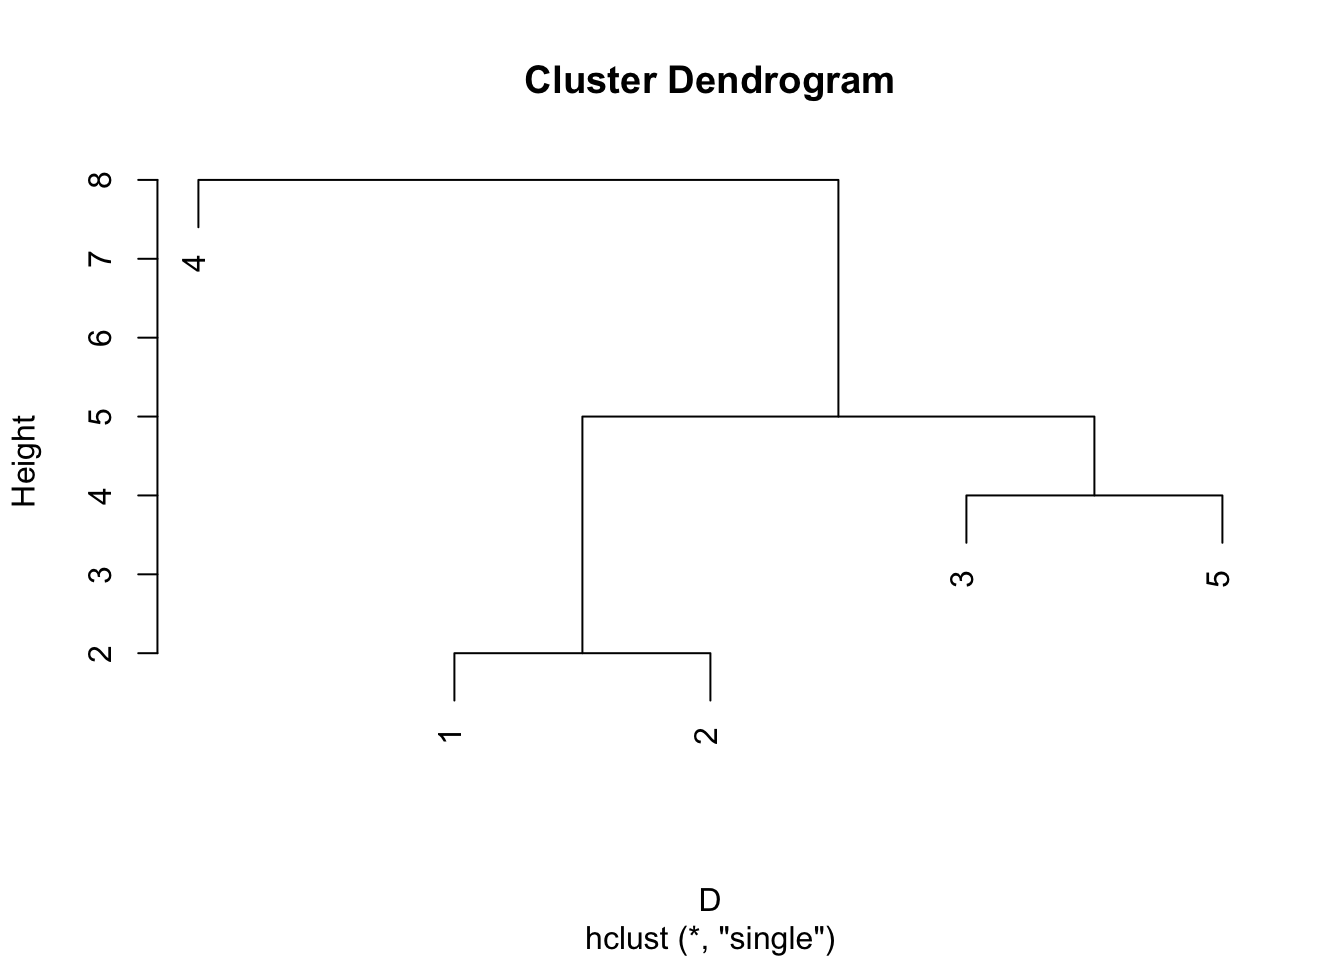
\includegraphics[width=1\linewidth]{03-matrix-decompositions_files/figure-latex/unnamed-chunk-13-1}

This is a \(512 \times 512\) colour image, meaning that there are three matrices \(\boldsymbol R, \boldsymbol B,\boldsymbol G\) of dimension \(512\times 512\)) giving the intensity of red, green, and blue for each pixel.
Naively storing this matrix requires 5.7Mb.

We can compute the SVD of the three colour intensity matrices, and the view the image that results from using reduced rank versions \(\boldsymbol B_k, \boldsymbol G_k, \boldsymbol R_k\) instead (as in Equation \eqref{eq:svdreduced}). The image below is formed using \(k=5, 30, 100\), and \(300\) basis vectors.

\begin{Shaded}
\begin{Highlighting}[]
\NormalTok{svd_image <-}\StringTok{ }\ControlFlowTok{function}\NormalTok{(im,k)\{}
\NormalTok{  s <-}\StringTok{ }\KeywordTok{svd}\NormalTok{(im)}
\NormalTok{  Sigma_k <-}\StringTok{ }\KeywordTok{diag}\NormalTok{(s}\OperatorTok{$}\NormalTok{d[}\DecValTok{1}\OperatorTok{:}\NormalTok{k])}
\NormalTok{  U_k <-}\StringTok{ }\NormalTok{s}\OperatorTok{$}\NormalTok{u[,}\DecValTok{1}\OperatorTok{:}\NormalTok{k]}
\NormalTok{  V_k <-}\StringTok{ }\NormalTok{s}\OperatorTok{$}\NormalTok{v[,}\DecValTok{1}\OperatorTok{:}\NormalTok{k]}
\NormalTok{  im_k <-}\StringTok{ }\NormalTok{U_k }\OperatorTok\StringTok{ }\NormalTok{Sigma_k }\OperatorTok\StringTok{ }\KeywordTok{t}\NormalTok{(V_k)}
   \CommentTok{## the reduced rank SVD produces some intensities <0 and >1. }
  \CommentTok{# Let's truncate these}
\NormalTok{  im_k[im_k}\OperatorTok{>}\DecValTok{1}\NormalTok{]=}\DecValTok{1}
\NormalTok{  im_k[im_k}\OperatorTok{<}\DecValTok{0}\NormalTok{]=}\DecValTok{0}
  \KeywordTok{return}\NormalTok{(im_k)}
\NormalTok{\}}

\KeywordTok{par}\NormalTok{(}\DataTypeTok{mfrow=}\KeywordTok{c}\NormalTok{(}\DecValTok{2}\NormalTok{,}\DecValTok{2}\NormalTok{), }\DataTypeTok{mar=}\KeywordTok{c}\NormalTok{(}\DecValTok{1}\NormalTok{,}\DecValTok{1}\NormalTok{,}\DecValTok{1}\NormalTok{,}\DecValTok{1}\NormalTok{))}

\NormalTok{pepprssvd<-}\StringTok{ }\NormalTok{peppers}
\ControlFlowTok{for}\NormalTok{(k }\ControlFlowTok{in} \KeywordTok{c}\NormalTok{(}\DecValTok{4}\NormalTok{,}\DecValTok{30}\NormalTok{,}\DecValTok{100}\NormalTok{,}\DecValTok{300}\NormalTok{))\{}
\NormalTok{  svds<-}\KeywordTok{list}\NormalTok{()}
  \ControlFlowTok{for}\NormalTok{(ii }\ControlFlowTok{in} \DecValTok{1}\OperatorTok{:}\DecValTok{3}\NormalTok{) \{}
\NormalTok{    pepprssvd[,,ii]<-}\KeywordTok{svd_image}\NormalTok{(peppers[,,ii],k)}
\NormalTok{  \}}
  \KeywordTok{plot}\NormalTok{(}\KeywordTok{as.raster}\NormalTok{(pepprssvd))}
\NormalTok{\}}
\end{Highlighting}
\end{Shaded}

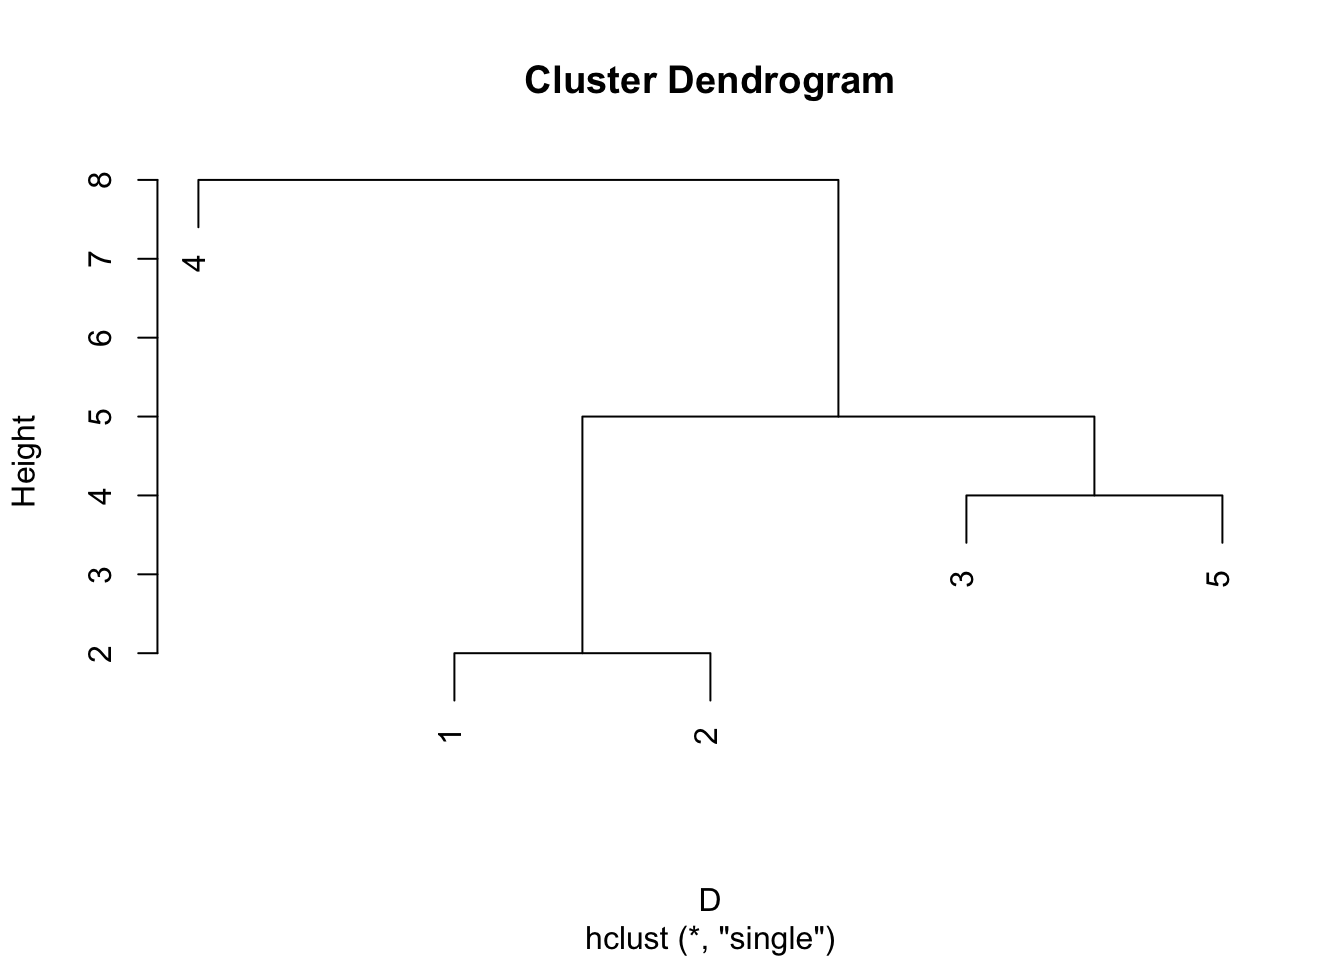
\includegraphics[width=1\linewidth]{03-matrix-decompositions_files/figure-latex/unnamed-chunk-14-1}

You can see that for \(k=30\) we have a reasonable approximation, but with some errors. With \(k=100\) it is hard to spot the difference with the original. The size of the four compressed images is 45Kb, 345Kb, 1.1Mb and 3.4Mb.

You can see further demonstrations of image compression with the SVD \href{http://timbaumann.info/svd-image-compression-demo/}{here}.

We will see much more of the SVD in later chapters.

\bibliography{book.bib,packages.bib}

\end{document}
